\documentclass{article}

\usepackage{neurips_2026}
\usepackage[utf8]{inputenc}
\usepackage[T1]{fontenc}
\usepackage{hyperref}
\usepackage{url}
\usepackage{booktabs}
\usepackage{graphicx}
\usepackage{amsmath}
\usepackage{xcolor}
\usepackage{microtype}

\graphicspath{{figures/}{auto/}}

% Placeholder macro: any number not yet measured renders red with a dagger.
\newcommand{\ph}[1]{\textcolor{red}{\underline{#1}$^{\dagger}$}}

% AUTO-GENERATED numbers. Every quantity quoted in this paper resolves through
% autopilot/p8_make_assets.py, which reads only verified JSON artifacts. No
% number below is typed by hand, so prose, tables and figures cannot disagree.
% AUTO-GENERATED by autopilot/p8_make_assets.py - do not edit by hand
% Every number in the manuscript resolves through these macros.
\newcommand{\Ntest}{3000}
\newcommand{\Npos}{1466}
\newcommand{\Nneg}{1534}
\newcommand{\Nboot}{10{,}000}
\newcommand{\Nprobes}{23}
\newcommand{\AUCRandomEpFifty}{0.8641}
\newcommand{\CIloRandomEpFifty}{0.8510}
\newcommand{\CIhiRandomEpFifty}{0.8769}
\newcommand{\AUCOracleEpFifty}{0.8740}
\newcommand{\CIloOracleEpFifty}{0.8615}
\newcommand{\CIhiOracleEpFifty}{0.8862}
\newcommand{\AUCEnvelopeEpFifty}{0.8761}
\newcommand{\CIloEnvelopeEpFifty}{0.8635}
\newcommand{\CIhiEnvelopeEpFifty}{0.8879}
\newcommand{\DOracleRandomEpFifty}{+0.0099}
\newcommand{\DOracleRandomEpFiftyCI}{[+0.0051,\,+0.0149]}
\newcommand{\DOracleRandomEpFiftyP}{$<$0.0001}
\newcommand{\DOracleRandomEpFiftyQ}{0.0001}
\newcommand{\DEnvelopeRandomEpFifty}{+0.0120}
\newcommand{\DEnvelopeRandomEpFiftyCI}{[+0.0068,\,+0.0173]}
\newcommand{\DEnvelopeRandomEpFiftyP}{$<$0.0001}
\newcommand{\DEnvelopeRandomEpFiftyQ}{$<$0.0001}
\newcommand{\DOracleEnvelopeEpFifty}{-0.0020}
\newcommand{\DOracleEnvelopeEpFiftyCI}{[-0.0069,\,+0.0029]}
\newcommand{\DOracleEnvelopeEpFiftyP}{0.4114}
\newcommand{\DOracleEnvelopeEpFiftyQ}{0.4114}
\newcommand{\AUCRandomEpSeventyFive}{0.8723}
\newcommand{\CIloRandomEpSeventyFive}{0.8593}
\newcommand{\CIhiRandomEpSeventyFive}{0.8849}
\newcommand{\AUCOracleEpSeventyFive}{0.8836}
\newcommand{\CIloOracleEpSeventyFive}{0.8714}
\newcommand{\CIhiOracleEpSeventyFive}{0.8955}
\newcommand{\AUCEnvelopeEpSeventyFive}{0.8803}
\newcommand{\CIloEnvelopeEpSeventyFive}{0.8677}
\newcommand{\CIhiEnvelopeEpSeventyFive}{0.8922}
\newcommand{\DOracleRandomEpSeventyFive}{+0.0113}
\newcommand{\DOracleRandomEpSeventyFiveCI}{[+0.0063,\,+0.0164]}
\newcommand{\DOracleRandomEpSeventyFiveP}{$<$0.0001}
\newcommand{\DOracleRandomEpSeventyFiveQ}{$<$0.0001}
\newcommand{\DEnvelopeRandomEpSeventyFive}{+0.0080}
\newcommand{\DEnvelopeRandomEpSeventyFiveCI}{[+0.0028,\,+0.0132]}
\newcommand{\DEnvelopeRandomEpSeventyFiveP}{0.0025}
\newcommand{\DEnvelopeRandomEpSeventyFiveQ}{0.0045}
\newcommand{\DOracleEnvelopeEpSeventyFive}{+0.0033}
\newcommand{\DOracleEnvelopeEpSeventyFiveCI}{[-0.0013,\,+0.0079]}
\newcommand{\DOracleEnvelopeEpSeventyFiveP}{0.1491}
\newcommand{\DOracleEnvelopeEpSeventyFiveQ}{0.1677}
\newcommand{\AUCRandomEpHundred}{0.8746}
\newcommand{\CIloRandomEpHundred}{0.8618}
\newcommand{\CIhiRandomEpHundred}{0.8869}
\newcommand{\AUCOracleEpHundred}{0.8855}
\newcommand{\CIloOracleEpHundred}{0.8735}
\newcommand{\CIhiOracleEpHundred}{0.8971}
\newcommand{\AUCEnvelopeEpHundred}{0.8807}
\newcommand{\CIloEnvelopeEpHundred}{0.8683}
\newcommand{\CIhiEnvelopeEpHundred}{0.8926}
\newcommand{\DOracleRandomEpHundred}{+0.0109}
\newcommand{\DOracleRandomEpHundredCI}{[+0.0057,\,+0.0160]}
\newcommand{\DOracleRandomEpHundredP}{$<$0.0001}
\newcommand{\DOracleRandomEpHundredQ}{$<$0.0001}
\newcommand{\DEnvelopeRandomEpHundred}{+0.0062}
\newcommand{\DEnvelopeRandomEpHundredCI}{[+0.0010,\,+0.0113]}
\newcommand{\DEnvelopeRandomEpHundredP}{0.0199}
\newcommand{\DEnvelopeRandomEpHundredQ}{0.0299}
\newcommand{\DOracleEnvelopeEpHundred}{+0.0047}
\newcommand{\DOracleEnvelopeEpHundredCI}{[+0.0004,\,+0.0091]}
\newcommand{\DOracleEnvelopeEpHundredP}{0.0294}
\newcommand{\DOracleEnvelopeEpHundredQ}{0.0378}
\newcommand{\AUCAnatomyTwoEpFifty}{0.8654}
\newcommand{\DAnatomyTwoRandomEpFifty}{+0.0013}
\newcommand{\DAnatomyTwoRandomEpFiftyCI}{[-0.0054,\,+0.0082]}
\newcommand{\DAnatomyTwoRandomEpFiftyP}{0.7101}
\newcommand{\AUCCoverEpFifty}{0.8643}
\newcommand{\DCoverRandomEpFifty}{+0.0002}
\newcommand{\DCoverRandomEpFiftyCI}{[-0.0049,\,+0.0053]}
\newcommand{\DCoverRandomEpFiftyP}{0.9440}
\newcommand{\AUCAncestor}{0.8487}
\newcommand{\NBlack}{431}
\newcommand{\NWhite}{2318}
\newcommand{\NAsian}{251}
\newcommand{\NprobesRace}{19}
\newcommand{\WorstRaceCount}{19}
\newcommand{\BlackAUCOracle}{0.8472}
\newcommand{\BlackCIOracle}{[0.8100,\,0.8804]}
\newcommand{\WhiteAUCOracle}{0.8853}
\newcommand{\RaceGapOracle}{0.0382}
\newcommand{\GapRho}{+0.511}
\newcommand{\GapRhoP}{0.0255}
\newcommand{\SexGapRho}{-0.714}
\newcommand{\SexGapRhoP}{0.0006}
\newcommand{\NprobesSub}{19}
\newcommand{\SubGenderRho}{-0.714}
\newcommand{\SubGenderRhoP}{0.0006}
\newcommand{\SubGenderQ}{0.0042}
\newcommand{\SubGenderBranchRho}{-0.857}
\newcommand{\SubGenderBranchP}{0.0137}
\newcommand{\SubGenderGapMin}{0.0272}
\newcommand{\SubGenderGapMax}{0.0396}
\newcommand{\SubGenderWorst}{female}
\newcommand{\SubGenderWorstN}{19}
\newcommand{\SubRaceRho}{+0.511}
\newcommand{\SubRaceRhoP}{0.0255}
\newcommand{\SubRaceQ}{0.0595}
\newcommand{\SubRaceBranchRho}{+0.429}
\newcommand{\SubRaceBranchP}{0.3374}
\newcommand{\SubRaceGapMin}{0.0475}
\newcommand{\SubRaceGapMax}{0.0935}
\newcommand{\SubRaceWorst}{black}
\newcommand{\SubRaceWorstN}{19}
\newcommand{\SubEthnicityRho}{+0.351}
\newcommand{\SubEthnicityRhoP}{0.1408}
\newcommand{\SubEthnicityQ}{0.1971}
\newcommand{\SubEthnicityBranchRho}{+0.464}
\newcommand{\SubEthnicityBranchP}{0.2939}
\newcommand{\SubEthnicityGapMin}{0.0223}
\newcommand{\SubEthnicityGapMax}{0.0661}
\newcommand{\SubEthnicityWorst}{hispanic}
\newcommand{\SubEthnicityWorstN}{19}
\newcommand{\SubLanguageRho}{+0.275}
\newcommand{\SubLanguageRhoP}{0.2537}
\newcommand{\SubLanguageQ}{0.2537}
\newcommand{\SubLanguageBranchRho}{+0.786}
\newcommand{\SubLanguageBranchP}{0.0362}
\newcommand{\SubLanguageGapMin}{0.0518}
\newcommand{\SubLanguageGapMax}{0.0805}
\newcommand{\SubLanguageWorst}{other languages}
\newcommand{\SubLanguageWorstN}{15}
\newcommand{\SubMaritalRho}{-0.444}
\newcommand{\SubMaritalRhoP}{0.0570}
\newcommand{\SubMaritalQ}{0.0997}
\newcommand{\SubMaritalBranchRho}{-0.714}
\newcommand{\SubMaritalBranchP}{0.0713}
\newcommand{\SubMaritalGapMin}{0.0364}
\newcommand{\SubMaritalGapMax}{0.0654}
\newcommand{\SubMaritalWorst}{single}
\newcommand{\SubMaritalWorstN}{19}
\newcommand{\SubAgeRho}{+0.304}
\newcommand{\SubAgeRhoP}{0.2065}
\newcommand{\SubAgeQ}{0.2409}
\newcommand{\SubAgeBranchRho}{+0.357}
\newcommand{\SubAgeBranchP}{0.4316}
\newcommand{\SubAgeGapMin}{0.0487}
\newcommand{\SubAgeGapMax}{0.0704}
\newcommand{\SubAgeWorst}{$<$60}
\newcommand{\SubAgeWorstN}{18}
\newcommand{\SubSeverityRho}{-0.521}
\newcommand{\SubSeverityRhoP}{0.0222}
\newcommand{\SubSeverityQ}{0.0595}
\newcommand{\SubSeverityBranchRho}{-0.857}
\newcommand{\SubSeverityBranchP}{0.0137}
\newcommand{\SubSeverityGapMin}{0.1286}
\newcommand{\SubSeverityGapMax}{0.1400}
\newcommand{\SubSeverityWorst}{mild ($-6$,$-2$]}
\newcommand{\SubSeverityWorstN}{19}
\newcommand{\NbranchesSub}{7}
\newcommand{\SeverityGapSpread}{0.0114}
\newcommand{\SubAUCMin}{0.8483}
\newcommand{\SubAUCMax}{0.8855}
\newcommand{\SevRandomMild}{0.8164}
\newcommand{\SevRandomModerate}{0.9030}
\newcommand{\SevRandomSevere}{0.9525}
\newcommand{\SevOracleMild}{0.8301}
\newcommand{\SevOracleModerate}{0.9131}
\newcommand{\SevOracleSevere}{0.9588}
\newcommand{\SevEnvelopeMild}{0.8232}
\newcommand{\SevEnvelopeModerate}{0.9103}
\newcommand{\SevEnvelopeSevere}{0.9559}
\newcommand{\SevDeltaMild}{+0.0137}
\newcommand{\SevDeltaModerate}{+0.0102}
\newcommand{\SevDeltaSevere}{+0.0063}
\newcommand{\SevGapRandom}{0.1361}
\newcommand{\SevGapOracle}{0.1286}
\newcommand{\RaceRandomWhite}{0.8741}
\newcommand{\RaceRandomBlack}{0.8325}
\newcommand{\RaceRandomAsian}{0.9033}
\newcommand{\RaceOracleWhite}{0.8853}
\newcommand{\RaceOracleBlack}{0.8472}
\newcommand{\RaceOracleAsian}{0.9189}
\newcommand{\BlackGainOracle}{+0.0147}
\newcommand{\FTOracleMeanpool}{0.8947}
\newcommand{\FTRandomMeanpool}{0.8868}
\newcommand{\FTDelta}{+0.0079}
\newcommand{\FTOracleBest}{0.8947}
\newcommand{\FTRandomBest}{0.8878}
\newcommand{\FTDeltaBest}{+0.0069}


% ARM DISPLAY NAMES. Defined once so a rename is a one-line change and cannot
% drift between prose, tables and figure captions. \ArmBest is the strongest
% arm: it locates a retinal band by a per-column intensity centroid and uses NO
% segmentation model and NO ground-truth labels. Named for what it computes.
\newcommand{\ArmBest}{\textsc{centroid}}

\title{Where to Aim, Not How Much to Cover:\\
Segmentation-Free Anatomy Guidance for\\
Masked Predictive Pretraining on Retinal OCT}

\author{}

\begin{document}

\maketitle

\begin{abstract}
Masked predictive pretraining asks a model to reconstruct the representation of
hidden image regions. Which regions are hidden is a free design choice, and in
medical imaging there is an intuitive answer: hide the tissue that carries the
diagnosis. We test that intuition under tightly controlled conditions. Six
masking policies are continued from a single shared I-JEPA checkpoint on 3D
retinal OCT, differing in how predictor targets are placed, and
evaluated with a frozen linear-probe protocol for glaucoma classification
(FairVision, $N{=}\Ntest$). Each policy was continued once, so what follows
describes these runs rather than an expected ranking over retrainings.
\emph{Region} matters: aiming the same rectangles --- same shapes, sizes and
counts --- at retinal tissue rather than at the whole frame improves AUC by
$\DEnvelopeRandomEpFifty$ over unguided masking at the matched epoch, and a band
located by a first-order intensity statistic, using no segmentation model at all,
improves it by $\DOracleRandomEpHundred$ at epoch 100. Both arms exclude zero at
all three epochs. Anatomical \emph{precision} does not add. A policy that places
$97\%$ of masked patches on tissue, using a trained retinal segmentation model to
shape the targets, matches unguided masking at epoch 50 and falls \emph{below} it
by epoch 75, as does a coverage-constrained policy; carried to epoch 100 the
latter does not merely stall but peaks at epoch \CoverPeakEpoch{} and then
declines, and an audit found its targets are shortened after placement, so it
does not test aggressive coverage. Direct measurement of mask geometry across
600 slices shows the winner hides the \emph{least} anatomy of any guided policy:
anatomy says where to aim, not how much to cover. Nor are the null's background
targets wasted --- they are a genuine pretraining signal, even though background
contributes almost nothing to the classifier. A subgroup audit over
\NprobesSub{} probes finds the same worst-served group every time; every disease
stage improves with intervals excluding zero (largest for mild, $\SevDeltaMild$,
though the gains are not separated from one another), while among race groups
only the white subgroup's gain excludes zero. The difficulty ordering is
untouched: the severe-to-mild
gap stays within $\SeverityGapSpread$ of constant across every policy.
\end{abstract}

\section{Introduction}



Self-supervised learning has become the default route to representation quality
in medical imaging, where expert annotation is expensive and pathology is
rare~\citep{azizi2021big,zhou2023retfound,qiu2024visionfm}. Joint-embedding
predictive architectures such as I-JEPA~\citep{assran2023ijepa} learn by
predicting the \emph{representation} of masked target blocks from a visible
context block, avoiding pixel reconstruction and its bias toward high-frequency
detail~\citep{he2022mae,xie2022simmim}.

I-JEPA samples its targets geometrically: rectangles placed uniformly at random.
In natural images this is defensible, since informative content is spread
broadly across the frame. In a retinal OCT B-scan it is not obviously so. A
large fraction of the image is dark vitreous and background; the diagnostic
signal for glaucoma is concentrated in a thin band of retinal tissue. This
motivates an intuitive hypothesis, one that several recent methods
adopt~\citep{li2022semmae,li2024anatomask,wang2025maskwhatmatters,shi2022adios}:
\emph{direct the predictive objective at clinically meaningful anatomy rather
than at arbitrary image regions.}

We test this hypothesis directly and at several strengths. Rather than proposing
one anatomy-aware method and reporting that it beats a baseline, we construct a
\emph{ladder} of masking policies of increasing anatomical specificity --- from
unguided rectangles, through rectangles aimed at tissue, to ragged
targets whose shape follows the segmented retina --- and hold everything else
fixed. All arms continue from one shared pretrained checkpoint, use identical
optimiser, schedule, and effective batch size, and are evaluated under one
frozen-probe protocol.

Anatomy turns out to matter for \emph{where} targets are aimed rather than for
how much anatomy they cover. The
two policies whose targets track the segmented retina most faithfully are
statistically indistinguishable from unguided masking at epoch 50, and the one we
carried further falls significantly below it by epoch 75, while
two policies that merely place ordinary rectangles on tissue gain an order of
magnitude more. One earlier shaped policy did exceed its rectangle counterpart at
epoch 30, so the anatomy result is mixed rather than uniformly negative. The best
performer locates a band by a per-column intensity centroid and consults no
segmentation model.

\paragraph{Contributions.}
\begin{itemize}
\setlength{\itemsep}{0pt}\setlength{\parskip}{0pt}
\item A controlled six-arm study isolating masking policy in medical SSL, with a
      shared ancestor checkpoint and a single evaluation protocol (every probe
      fitted is listed in Appendix~\ref{app:allprobes}).
\item Evidence that in these runs guidance helps while anatomical precision does
      not reliably add to it, including the
      specific control --- rectangles aimed at retinal tissue --- that
      separates ``avoid background'' from ``target anatomy''.
\item Direct measurement of mask geometry for every policy on 600 slices,
      showing that the most anatomically precise policy is not the best
      performer, and
      an explicit accounting of the axes on which the anatomy arms are
      confounded.
\item A subgroup audit and a $10^{-5}$ reproduction of the headline result from
      public weights on different hardware and precision.
\end{itemize}

\section{Related work}

\paragraph{Masked image modelling and JEPAs.}
Masked autoencoders reconstruct pixels~\citep{he2022mae,xie2022simmim};
BEiT~\citep{bao2022beit} and iBOT~\citep{zhou2022ibot} predict discrete tokens;
data2vec~\citep{baevski2022data2vec} and I-JEPA~\citep{assran2023ijepa} predict
latent representations. Video and 3D extensions follow the same
template~\citep{bardes2024vjepa,chen2023mim3d,taleb20203dssl}. Recent analyses
question how much of the benefit derives from the masking distribution
itself~\citep{balestriero2025lejepa,he2025dseqjepa}.

\paragraph{Informed masking.}
A substantial line of work argues that \emph{what} is masked matters.
ADIOS~\citep{shi2022adios} learns an adversarial masking model;
SemMAE~\citep{li2022semmae} uses learned semantic parts;
AttMask~\citep{kakogeorgiou2022attmask} masks by attention;
HardPatches~\citep{wang2023hardpatches} and AutoMAE~\citep{chen2023automae}
target difficulty. In the medical domain, AnatoMask~\citep{li2024anatomask},
AnatomyMAE~\citep{ceballosarroyo2026anatomymae},
MSMAE~\citep{mao2023msmae}, and VasoMIM~\citep{huang2026vasomim} explicitly
steer masking toward anatomy, and \citet{wang2025maskwhatmatters} argue directly
for masking clinically relevant regions. Our study is a controlled test of that
family's central premise on one task.

\paragraph{Evidence that informed masking is not uniformly better.}
The picture is less one-sided than that suggests. The original masked-modelling
papers report that random sampling is hard to beat: MAE's ablation puts
random-75 at $73.5$ linear against block-75 at $63.9$~\citep{he2022mae}, and
SimMIM finds random beats its best block variant~\citep{xie2022simmim}. Among
informed schemes, AttMask sits within $0.2$
points of random~\citep{kakogeorgiou2022attmask}, AutoMAE ties MAE under full
fine-tuning~\citep{chen2023automae}, HPM gains only when randomness is retained
and \emph{loses} when restricted to the hardest patches~\citep{wang2023hpm}, and
attention-guided MAE underperforms MAE in the low-label
regime~\citep{sick2025attg}. Most directly, SemMAE's own ablation
shows that \emph{imperfect} semantic parts add nothing over no parts at
all~\citep{li2022semmae}, and \citet{guo2025mlomae} reproduce SemMAE below random
MAE, the deficit largest under frozen evaluation --- also our protocol.
\citet{chen2023automae} name the mechanism a ``patch selection
dilemma'': a slight foreground bias helps, but raising it too far starves the
encoder of the evidence it must predict from. The closest positive
precedent for our best policy is segmentation-free too:
\citet{lee2025hufgm} select foreground from normalised intensity alone and gain
across five 3D medical benchmarks (Appendix~\ref{app:counter} tabulates these).
That random masking is a strong baseline, and semantic guidance wins only
sometimes, is known and contested; we do not overturn that literature. We add a
controlled measurement of where a \emph{trained medical segmentation model}
falls on that spectrum, in a setting --- 3D retinal OCT, joint-embedding
prediction, frozen probe --- where we found no prior controlled comparison.

\paragraph{Retinal foundation models, OCT, and fairness.}
RETFound~\citep{zhou2023retfound}, VisionFM~\citep{qiu2024visionfm},
URFound~\citep{yu2024urfound}, and OCTCube~\citep{liu2026octcube} pretrain on
large retinal corpora; OCT-specific masked modelling is explored by
\citet{pissas2024octmim}. MIRAGE~\citep{morano2025mirage} provides multimodal
OCT segmentation and supplies the anatomical guidance used by several of our
arms, and deep glaucoma detection from OCT is
established~\citep{maetschke2019glaucoma,ran2019glaucoma,noury2022glaucoma}.
Performance disparities across demographic groups are widely
documented~\citep{seyyedkalantari2021underdiagnosis,larrazabal2020gender,gichoya2022race};
FairVision~\citep{luo2024fairvision} and Harvard-GF~\citep{luo2024harvardgf}
provide OCT data with demographic attributes, and
FairMedFM~\citep{jin2024fairmedfm} and \citet{shi2025equitable} benchmark
fairness for medical foundation models.

\section{Method: a ladder of masking policies}
\label{sec:policies}

\subsection{Background}

I-JEPA samples from the token grid of an image a context block and $M$ target
blocks, which need not cover it. A context encoder embeds the visible tokens; a predictor maps that
embedding plus positional queries to predicted representations of the target
tokens; an exponential-moving-average target encoder supplies the regression
targets. With a $16{\times}16$ token grid the design choice we vary is which of
the 256 cells become targets.

\subsection{The six policies}

All policies produce $M{=}4$ target blocks and one context block under identical
scale and aspect-ratio ranges. The rectangle arms differ only in placement.

\begin{description}
\setlength{\itemsep}{1pt}\setlength{\parskip}{0pt}
\item[\textsc{random} (null).] Stock I-JEPA multiblock. Four rectangles placed
  uniformly at random anywhere in the grid. No image content is consulted.

\item[\textsc{envelope} (random-within-retina).] Identical rectangles ---
  same shape, size and count as \textsc{random} --- but rejection-sampled onto
  the retinal envelope predicted by MIRAGE~\citep{morano2025mirage}. Only
  \emph{location} changes. This is the control that separates ``stop wasting
  targets on background'' from ``target anatomy specifically''.

\item[\ArmBest{} (segmentation-free).] A band whose vertical position is
  located per slice by a per-column intensity-weighted row centroid, smoothed
  across columns. It adapts to the retina's position and curvature from a
  first-order intensity statistic, with no segmentation model and no ground-truth
  annotation of any kind.

\item[\textsc{anatomy-v1} / \textsc{anatomy-v2}.] Ragged connected components
  grown on the MIRAGE score map, so target \emph{shape} follows tissue rather
  than being rectangular. v2 additionally bridges diagonal adjacencies.

\item[\textsc{cover} $f$.] Targets chosen greedily to cover the anatomy subject
  to a hard floor leaving a fraction $f$ of tissue visible in the context. We
  pretrain $f{=}0.21$. An implementation defect means the delivered masks never
  reach $f$ (Appendix~\ref{app:covbug}).
\end{description}

Figure~\ref{fig:policies} shows all six on the same B-scans.


\begin{figure}[t]
\centering
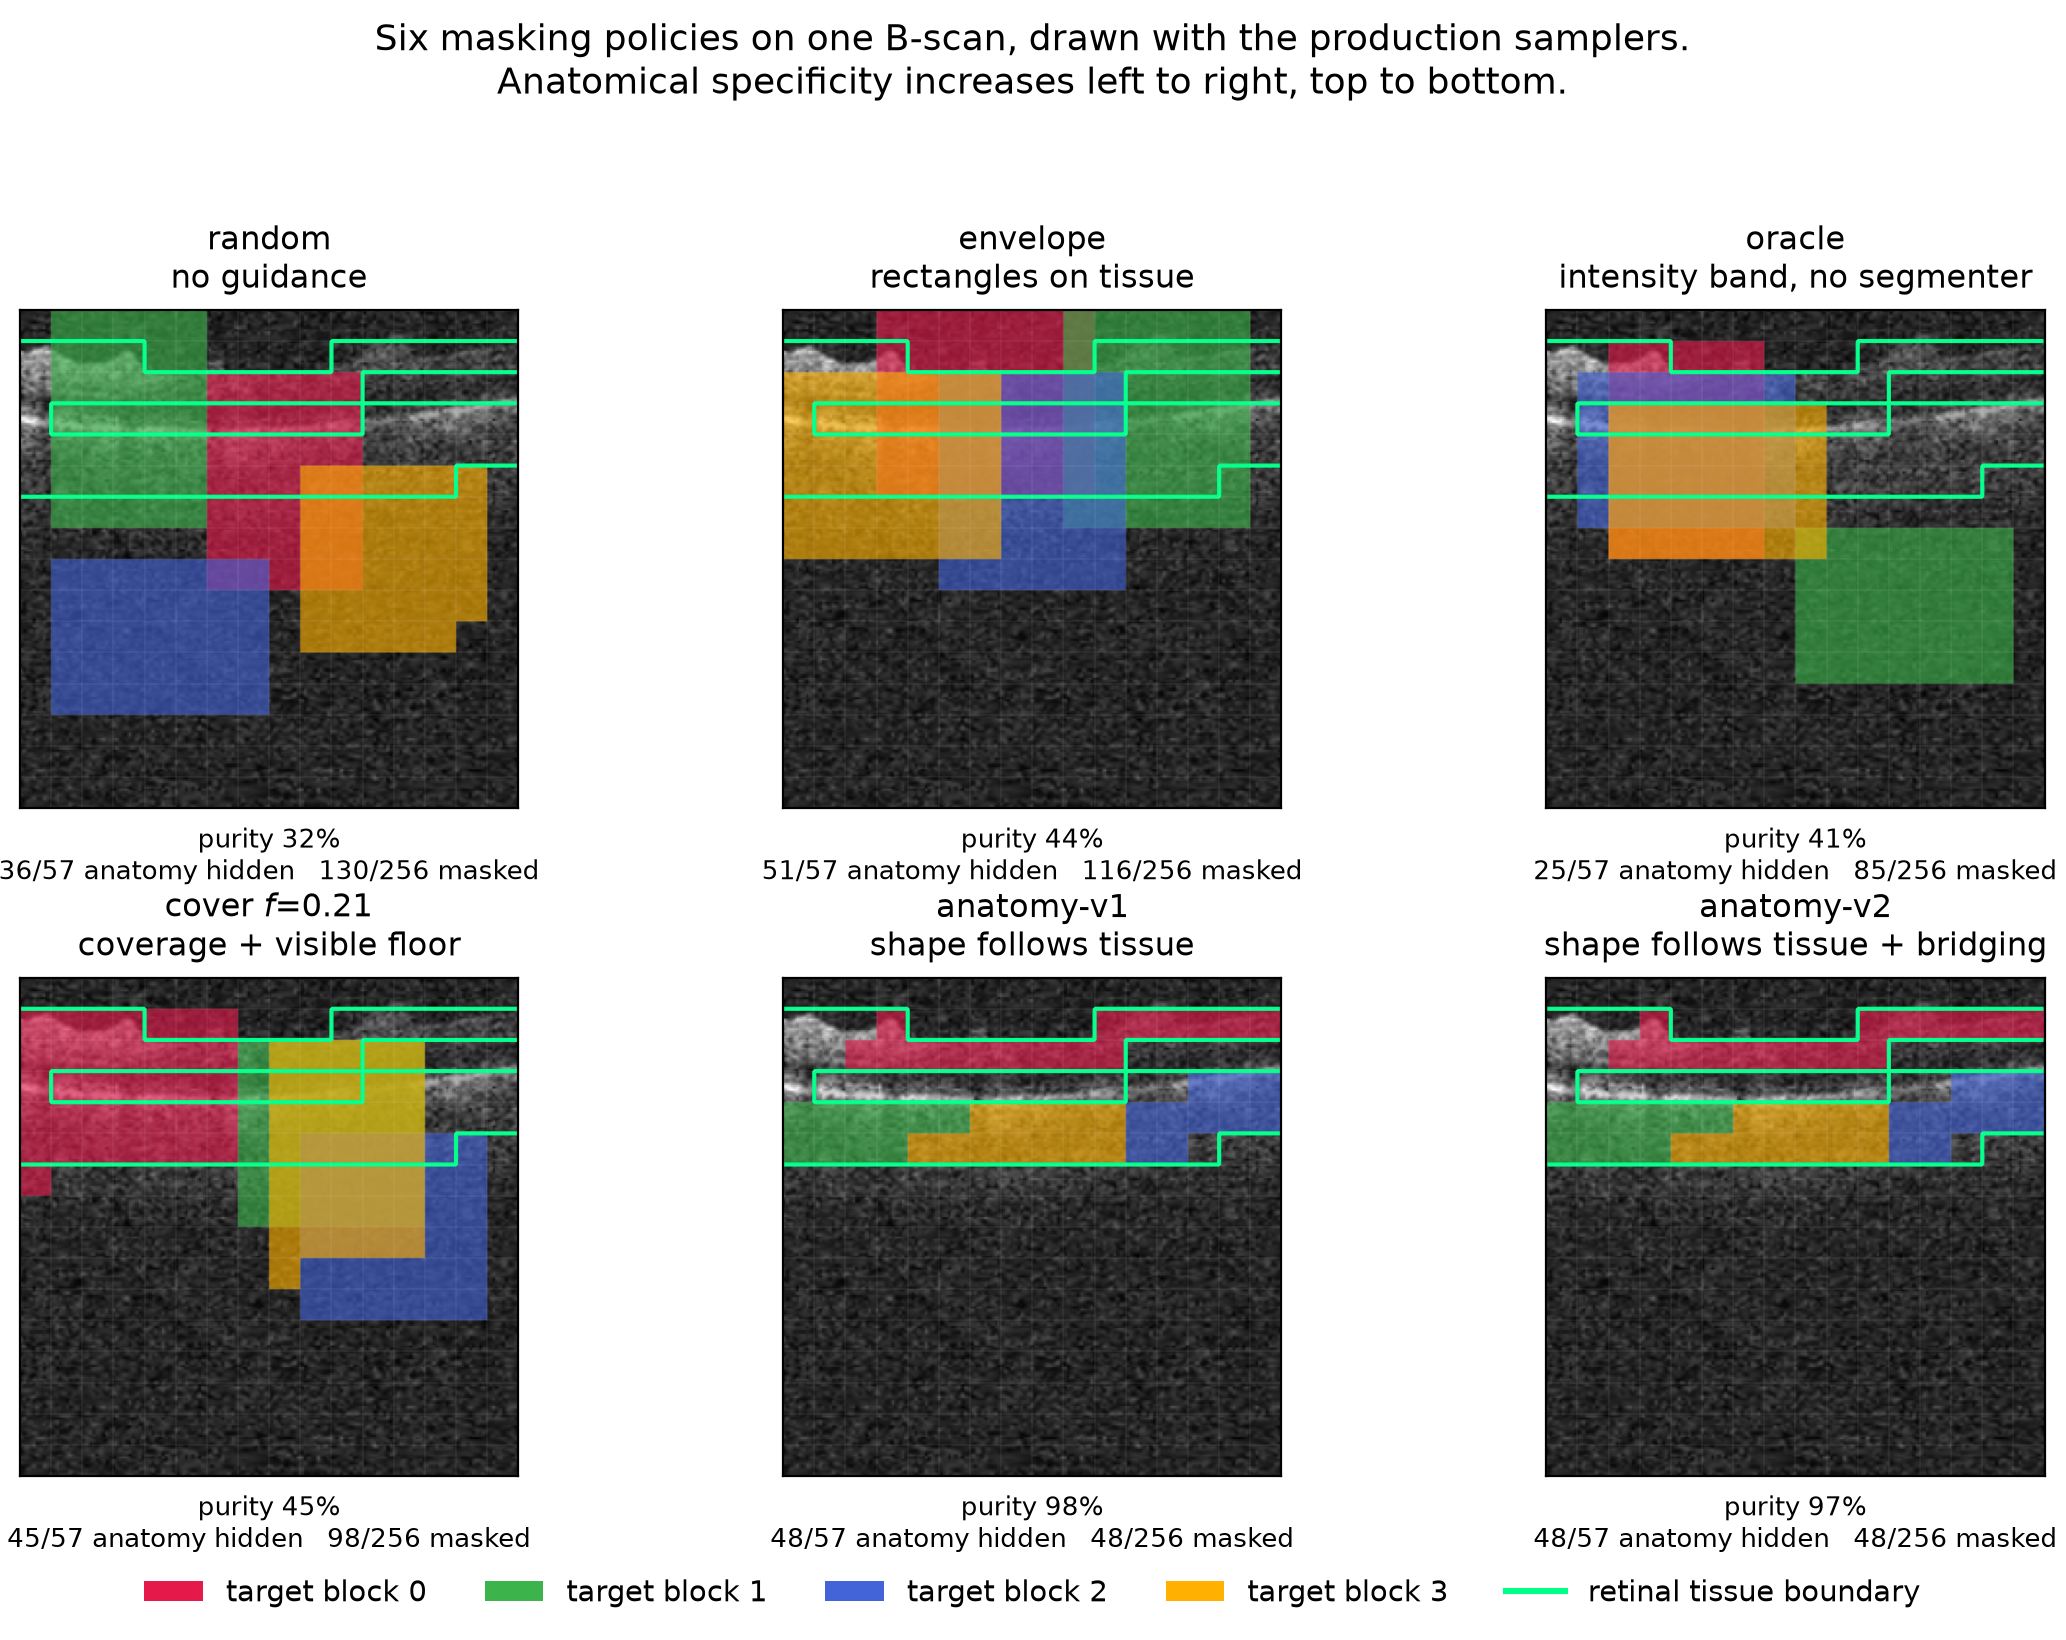
\includegraphics[width=0.53\linewidth]{fig1_policies_compact.png}
\caption{The six masking policies on one identical B-scan, drawn with the
production samplers. Each target block has its own colour; the green
contour is the anatomy reference. Anatomical specificity increases along the
ladder: \textsc{envelope} and \textsc{cover} place rectangles on tissue, while
the anatomy arms grow targets that trace the retina almost exactly. Downstream
AUC does not increase with that specificity (Table~\ref{tab:main});
Figure~\ref{fig:policies5} repeats this over five B-scans.}
\label{fig:policies}
\end{figure}

\subsection{Hypotheses}

The ladder yields three testable statements:

\begin{description}
\setlength{\itemsep}{1pt}\setlength{\parskip}{0pt}
\item[H1] \emph{Avoiding background helps.} \textsc{envelope} $>$ \textsc{random}.
\item[H2] \emph{Anatomical precision helps further.} anatomy arms $>$
  \textsc{envelope}.
\item[H3] \emph{Any benefit is due to anatomical targeting, not to incidental
  changes in mask area, target count, or context size.}
\end{description}

\section{Experimental setup}
\label{sec:setup}

\paragraph{Data.} FairVision~\citep{luo2024fairvision} glaucoma OCT volumes.
Each volume is a 3D scan resampled to 100 B-scans of $256{\times}256$ after
transform. The label is a binary glaucoma diagnosis. Splits are fixed and
patient-disjoint as released; downstream evaluation uses a held-out test split of
$N{=}3000$ volumes (1466 positive / 1534 negative), seed 42, fixed loader order.
No test volume is used to fit or select the probe head, which is selected on a
separate validation split; the study's choices of policy, checkpoint, analysis
and stopping horizon were made after repeated inspection of that same test split
(Section~\ref{sec:limits}). Labels are byte-identical
across arms, so any two arms are paired-comparable on the same cases. Self-reported
demographic attributes are used only for the subgroup
analysis in Section~\ref{sec:subgroup} and never as model inputs.

\paragraph{Pretraining.} Patch-level I-JEPA, ViT-Base, $256{\times}256$ crops,
patch size 16, predictor depth 6, EMA target encoder. \textbf{Every arm resumes
from the same epoch-25 checkpoint} and continues with identical optimiser,
learning-rate and weight-decay schedules, and effective batch size (512 for all
arms). Guidance is ramped linearly from epoch 25 to 30 and held at full strength
thereafter. Within the rectangle family the \emph{only} difference between arms
is the mask sampler (Section~\ref{sec:policies}); the anatomy family
additionally differs in collation, and
we quantify that in Section~\ref{sec:results}.

Arms differ in how far they were carried.
\textsc{random}, \ArmBest{} and \textsc{envelope} reach epoch 100.
\textsc{anatomy-v2} reaches epoch 75 (its epoch-75 and epoch-92 probes under an
earlier target-precision splice are excluded and replaced by a clean fp32
continuation, Appendix~\ref{app:excluded}); we stopped that arm having seen its
epoch-75 deficit, which is a selective stopping horizon and a real weakness ---
a trajectory can recover, and its epoch-100 value is unmeasured, not known to be
worse.
\textsc{anatomy-v1} has only epoch 30. \textsc{cover} $f{=}0.21$ reaches epoch
100, with an extra probe at its epoch-73 peak. Epoch 50 is therefore the only
epoch at which
five policies are simultaneously available, and it carries every cross-policy
comparison that involves the anatomy or coverage arms.

\paragraph{Evaluation.} The encoder is frozen. Per-slice features are
mean-pooled over the volume, followed by LayerNorm and a linear head. The head is
selected by validation AUC and reported on the held-out test split. We report
paired bootstrap confidence intervals over test volumes (\Nboot{} resamples,
stratified by class, the same resampled index set applied to every arm) and
DeLong tests for correlated ROC curves~\citep{delong1988roc}, both of which are
valid here because all arms are evaluated on the same cases in the same order.
Each test volume is a distinct subject, so case-level resampling is already
subject-level and no cluster correction is
required~\citep{obuchowski1997clusteredroc,rutter2000clusterbootstrap}. We follow
\citet{maierhein2024metricsreloaded} in reporting the operating-point metrics
alongside AUC rather than AUC alone (Appendix~\ref{app:operating}).

\paragraph{Numerical precision.} The probe harness
defaults to mixed precision. The \textsc{random}, \ArmBest{} and
\textsc{envelope} long-horizon probes were fitted under that default (fp16);
the \textsc{anatomy-v1}, \textsc{anatomy-v2}, \textsc{cover} and ancestor probes
were fitted with autocast explicitly disabled (fp32). Protocol is therefore not
uniform across probes, so we partition the comparisons: all headline contrasts in
Table~\ref{tab:main} are drawn from arms sharing both epoch \emph{and}
precision, and any contrast that would cross the precision boundary is marked
as such and excluded from headline claims. Section~\ref{sec:precision} measures
the precision effect.

\section{Results}
\label{sec:results}

Each policy was pretrained once, so the intervals below are sampling error over
test subjects, not seed-to-seed variance (Section~\ref{sec:limits}).

\subsection{Region matters: where you aim beats not aiming at all}

\begin{table}[t]
\centering
\caption{Frozen MeanPool probe, FairVision test ($N{=}\Ntest$, \Npos{} positive).
All arms continue from one epoch-25 ancestor (AUC $\AUCAncestor$). $\Delta$ is
versus \textsc{random} at the \emph{matched} epoch. The upper block is
precision-matched (fp16 throughout) and carries every headline claim; the lower
block is fp32, each $\Delta$ taken against an fp32 null re-probed at the same
epoch, so it is matched on both epoch and precision. The measured fp16/fp32
gap is at most $2\times10^{-4}$ (Appendix~\ref{app:fp32}).}
\label{tab:main}
\footnotesize
\setlength{\tabcolsep}{4pt}
\begin{tabular}{llcccccc}
\toprule
& & \multicolumn{2}{c}{epoch 50} & \multicolumn{2}{c}{epoch 75} & \multicolumn{2}{c}{epoch 100} \\
\cmidrule(lr){3-4}\cmidrule(lr){5-6}\cmidrule(lr){7-8}
policy & guidance signal & AUC & $\Delta$ & AUC & $\Delta$ & AUC & $\Delta$ \\
\midrule
\textsc{random}   & none (null)                      & \AUCRandomEpFifty  & ---                              & \AUCRandomEpSeventyFive  & ---                              & \AUCRandomEpHundred  & ---  \\
\textsc{envelope} & segmenter (location only)        & \AUCEnvelopeEpFifty & $\mathbf{\DEnvelopeRandomEpFifty}$ & \AUCEnvelopeEpSeventyFive & $\mathbf{\DEnvelopeRandomEpSeventyFive}$ & \AUCEnvelopeEpHundred & $\mathbf{\DEnvelopeRandomEpHundred}$ \\
\ArmBest{}   & intensity centroid, no segmenter & \AUCOracleEpFifty   & $\mathbf{\DOracleRandomEpFifty}$   & \AUCOracleEpSeventyFive   & $\mathbf{\DOracleRandomEpSeventyFive}$   & \textbf{\AUCOracleEpHundred} & $\mathbf{\DOracleRandomEpHundred}$ \\
\midrule
\textsc{anatomy-v2} & segmenter (target shape) & \TAUCAnatomyTwoEpFifty & \TAnatomyTwoRandomEpFifty & \TAUCAnatomyTwoEpSeventyFive & \TAnatomyTwoRandomEpSeventyFive & \TAUCAnatomyTwoEpHundred & \TAnatomyTwoRandomEpHundred \\
\textsc{cover} $f{=}.21$ & segmenter (coverage) & \TAUCCoverEpFifty & \TCoverRandomEpFifty & \TAUCCoverEpSeventyFive & \TCoverRandomEpSeventyFive & \TAUCCoverEpHundred & \TCoverRandomEpHundred \\
\bottomrule
\end{tabular}
\end{table}


Table~\ref{tab:main} gives the main comparison, Table~\ref{tab:contrasts} in
Appendix~\ref{app:contrasts} the full paired inference for all nine
precision-matched contrasts, and Figure~\ref{fig:traj} the trajectories.

\textbf{H1 holds, and the study's cleanest control carries it.}
\textsc{envelope} differs from the unguided null in \emph{location alone} ---
same rectangle shapes, sizes and counts, rejection-sampled onto the retinal
envelope instead of the whole frame. Moving them onto tissue is worth
$\DEnvelopeRandomEpFifty$ AUC at epoch 50, and \ArmBest{}, a band located from
a first-order intensity statistic with no segmentation model anywhere, is worth
$\DOracleRandomEpHundred$ at epoch 100. Every \textsc{envelope} and \ArmBest{}
interval excludes zero at all three epochs, and all six contrasts survive
Benjamini--Hochberg correction over that family of nine ($q \leq
\DEnvelopeRandomEpHundredQ$; Table~\ref{tab:contrasts},
Figure~\ref{fig:traj}b). Region is a real design variable.

Aiming is not containment: the rectangles are large, so fewer than half of
\textsc{envelope}'s masked cells land on tissue (Table~\ref{tab:geom}). Guidance
changes where the predictor is repeatedly sent, not what it is forbidden to see.
Why the unguided null nonetheless stays close has an answer of its own
(Section~\ref{sec:results-bg}).

\begin{figure}[t]
\centering
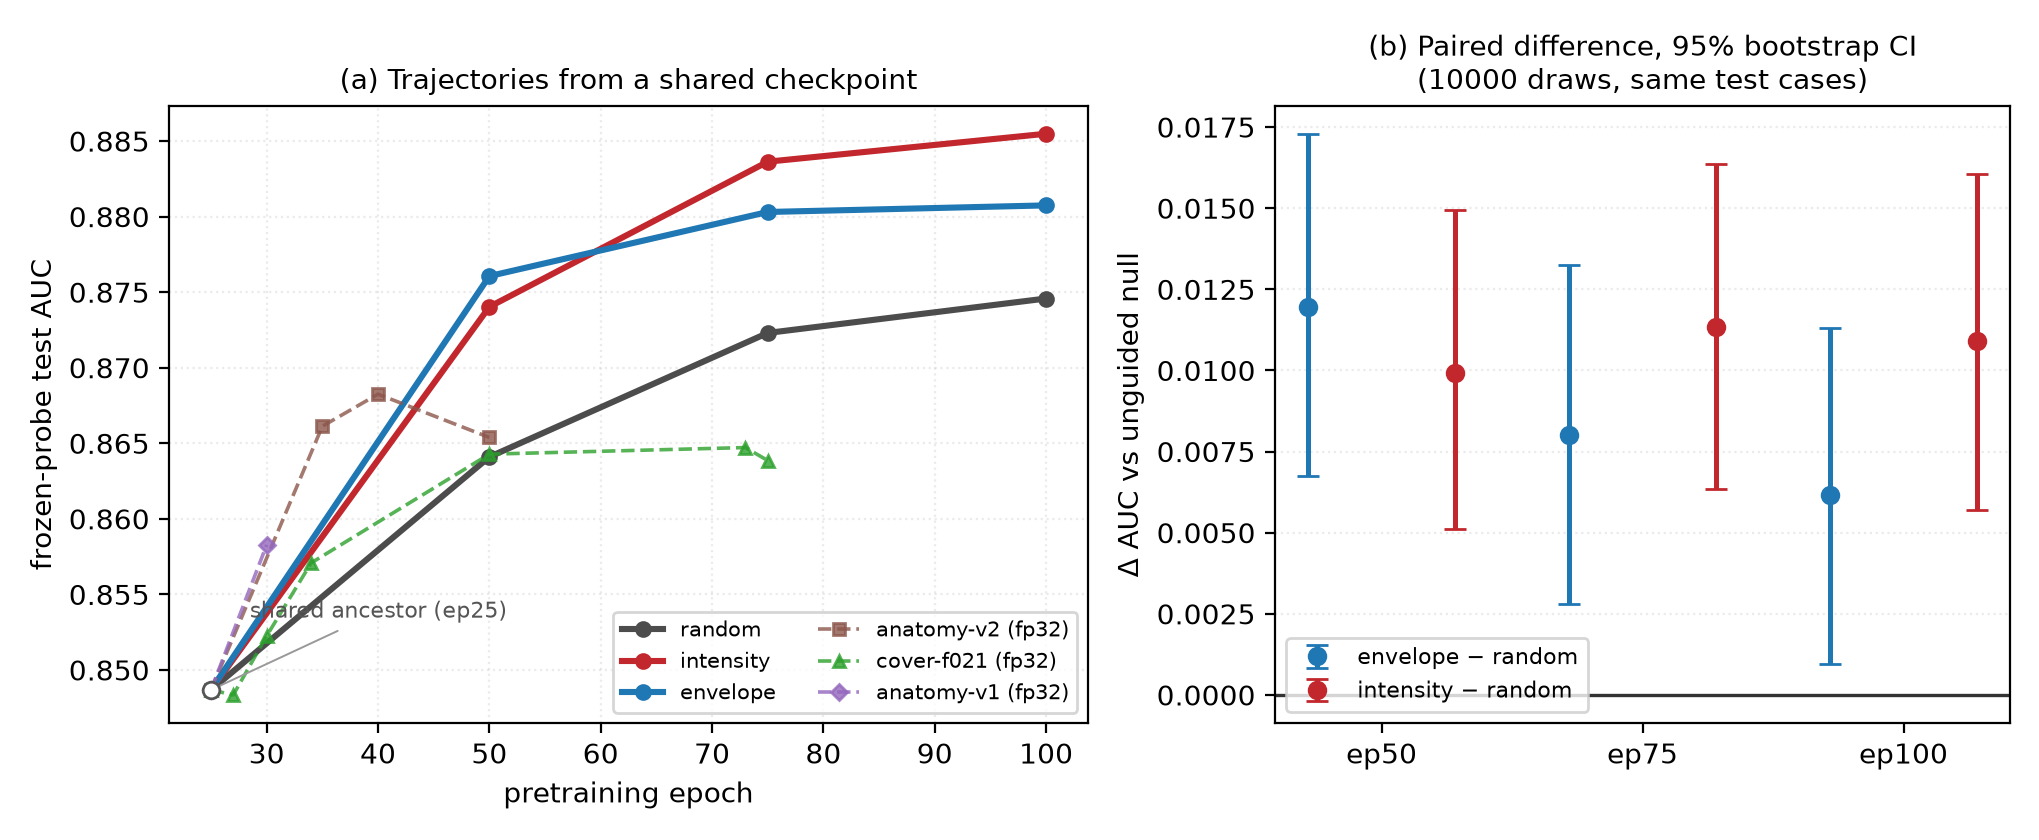
\includegraphics[width=0.78\linewidth]{fig_trajectories_ci.png}
\caption{\textbf{(a)} Frozen-probe test AUC against pretraining epoch. All arms
fork from the same epoch-25 checkpoint (open circle). Solid lines are the
precision-matched fp16 family; dashed lines are fp32
arms and must not be compared vertically against the solid lines.
\textbf{(b)} The actual inference: paired differences against the unguided null
on identical test cases, with \Nboot-resample bootstrap intervals. Every
\textsc{envelope} and \ArmBest{} interval excludes zero; \textsc{cover} straddles
zero at epoch 50 and is negative thereafter. Paired differences are plotted
rather than per-arm error bars: marginal intervals carry between-case variance
that cancels in a pairing and would understate the evidence.}
\label{fig:traj}
\end{figure}

\textbf{Precision beyond location does not add, and the evidence is mixed rather
than uniformly negative.} H2 predicts that the anatomy arms exceed
\textsc{envelope}. Tested directly at the matched epoch 50, \textsc{anatomy-v2}
sits $\DAnatomyTwoEnvelopeEpFifty$ \emph{below} \textsc{envelope} (CI
$\DAnatomyTwoEnvelopeEpFiftyCI$). At epoch 30, however, \textsc{anatomy-v1} sits
$\DAnatomyOneEnvelopeEpThirty$ \emph{above} it (CI
$\DAnatomyOneEnvelopeEpThirtyCI$). These are different implementations at
different epochs, so we do not read either as settling H2; what the pair rules
out is a uniform advantage for anatomical precision, not the possibility that
some shaped policy helps somewhere. Nor is \textsc{anatomy-v2} or \textsc{cover}
\emph{worse} than the null
at the matched epoch: both sit within a paired interval that comfortably contains
zero (Figure~\ref{fig:traj}b). The data rule out monotone improvement with
anatomical precision, not harm.

\paragraph{Carried to epoch 100 the coverage arm degrades.}
\textsc{cover} is the only policy that uses the segmenter to choose \emph{how
much} to hide, and carried to the full horizon it produces the study's one
\emph{negative} result. It climbs normally to epoch 50, peaks at epoch
$\CoverPeakEpoch$, then \emph{falls}, losing $\DCoverPeakToHundred$ from its own
peak ($p\,\DCoverPeakToHundredP$) while the unguided null keeps improving
(Figure~\ref{fig:traj}); its gap against the null widens monotonically across the
three matched epochs (Table~\ref{tab:main}).

We cannot read this as evidence that high coverage is harmful. An audit found
that the collator shortens predictor targets \emph{after} \textsc{cover} chooses
its placement, so its delivered masks hide \emph{less} anatomy than
\textsc{envelope}'s (Table~\ref{tab:geom}, Figure~\ref{fig:maskstats}) and the
arm never realised the coverage it was configured for;
Appendix~\ref{app:covbug} gives the full account.

\textbf{The strongest policy consults no segmentation model.} \ArmBest{} finds
its band from a per-column intensity centroid: no model and no annotation. Its
margin over the null is the largest at epoch 100 and does not decay with
training, whereas \textsc{envelope}'s does
(Table~\ref{tab:main}), and it exceeds the segmenter-guided \textsc{envelope} arm
at epoch 100 by $\DOracleEnvelopeEpHundred$ (CI $\DOracleEnvelopeEpHundredCI$),
though the two are indistinguishable at epochs 50 and 75.

\subsection{Aim, not coverage}
\label{sec:results-h3}

\begin{table}[t]
\centering
\caption{Measured mask geometry, 600 training slices, production samplers.
``purity'' is the fraction of masked cells lying on tissue; ``loss slots'' is the
number of predictor target \emph{cells} entering the loss, summed over the $M$
targets. AUC is quoted at the
\emph{matched} epoch 50, so the geometry-to-AUC association is not read across
mixed epochs.}
\label{tab:geom}
\footnotesize
\begin{tabular}{lcccccc}
\toprule
policy & anatomy hidden & purity & mask ratio & context kept & loss slots & AUC @ep50 \\
\midrule
\textsc{random}   & 54.0\% & 31.5\% & 44.5\% & 41.9\% & 159.9 & \AUCRandomEpFifty \\
\ArmBest{}   & 62.1\% & 40.0\% & 40.3\% & 45.5\% & 159.0 & \AUCOracleEpFifty \\
\textsc{envelope} & 77.6\% & 43.3\% & 46.5\% & 40.6\% & 159.7 & \textbf{\AUCEnvelopeEpFifty} \\
\textsc{cover}    & 73.5\% & 44.2\% & 43.2\% & 43.2\% & 159.1 & \AUCCoverEpFifty \\
\textsc{anatomy-v2} & 79.9\% & \textbf{97.1\%} & 21.3\% & 67.7\% & 64.0 & \AUCAnatomyTwoEpFifty \\
\bottomrule
\end{tabular}
\end{table}

To see what the policies actually deliver we ran each production sampler on 600
training slices and measured the realised masks (Table~\ref{tab:geom},
Figures~\ref{fig:paradox} and~\ref{fig:ladder}; provenance in
Appendix~\ref{app:geomprov}). Two observations follow.

First, \textbf{anatomy tells you where to aim, not how much to cover}. Of the
four guided arms the best performer hides the \emph{least} anatomy, while the arm
that hides the most --- masking almost nothing but tissue, at $97.1\%$ purity ---
does not separate from the null (Table~\ref{tab:geom}). What \ArmBest{} does
instead is leave more visible: it retains more context than any other rectangle
arm, and the background stays maskable. Rank correlations over these
arms are positive for both anatomy hidden and purity, but at $n{=}4$--$5$ arms
they resolve nothing in either direction and we draw no inference from them.
Occlusion attribution on the fine-tuned probes is correspondingly diffuse
(Appendix~\ref{app:interp}).

Second, \textbf{the anatomy arms are confounded on several axes simultaneously}.
\textsc{anatomy-v2} retains more context still, but it also hides far less of the
grid and collapses to
$64$ predictor loss slots against about $159$ for every rectangle arm
(Table~\ref{tab:geom}, Figure~\ref{fig:geom}) --- a much easier prediction task. They and \textsc{cover}
also differ from \textsc{envelope} in guide provenance
(Appendix~\ref{app:repro}). Any of these could
account for its deficit without invoking target shape at all. \textbf{H3 is
therefore not identified by this design}, and we do \emph{not} claim that
irregular target shape is harmful.

These are not consequences of blob geometry: the anatomy arms resample
every target to a fixed $K{=}16$ cells, so $4\times16=64$ loss slots follows by
construction, while the rectangle arms do not set $K$. The two families are
collated differently, which weakens ``everything else held fixed'' for the
anatomy-versus-rectangle comparison specifically; contrasts within the rectangle
family are unaffected (Appendix~\ref{app:covbug}).

\subsection{Background matters --- for pretraining, not for the classifier}
\label{sec:results-bg}

Unguided masking spends most of its targets on background, and they are not
wasted --- the most surprising result in the study. At epoch 100 the null's
predictor beats a per-position, no-context reference by $0.680$ on
\emph{background} targets, \emph{above} its $0.633$ on anatomy: predicting a
background token takes more than knowing where it sits, even though such tokens
start out nearly pure position ($90.8\%$ of across-position input variance there
comes from \texttt{pos\_embed}, against $40.8\%$ at tissue). Pretraining spends
real capacity on them, and background self-similarity falls from $0.784$
untrained to $0.346$.
Yet almost none of it reaches the classifier. Pooled background features are $95.2\%$
linearly reconstructible from pooled anatomy features; residualised, background
predicts glaucoma at test AUC $0.5515$ --- barely above chance, though the
interval excludes it --- and appending it to anatomy
\emph{lowers} test AUC for the null arm. That split --- a useful
\emph{pretraining} target, a near-useless \emph{classification} feature --- is why
unguided masking is such a strong baseline, and why aiming at tissue buys a gain
that is real but bounded. The mechanism is described rather than established:
the two controls that would settle it were not run (Appendix~\ref{app:bg}).

\subsection{The advantage concentrates where labels are scarce}
\label{sec:labeleff}

A masking policy that only helps when labels are plentiful is of limited
clinical use, so we withdrew supervision and re-fitted the same probe. Protocol
and label subsets are held fixed --- the subsampling seed depends on the fraction
and repeat but never on the arm --- and, across all four arms in this sweep, the
full-supervision fits reproduce their corresponding epoch-100 entries in
Table~\ref{tab:main} to within $0.0009$. The observed margin is larger with
fewer labels: at $5\%$ of the labelled set ($n{=}\LENFive$) \ArmBest{} leads the null by
$\LEGapFive$, against $\LEGapHundred$ at full supervision, more than four times
the advantage. Whether the gap genuinely widens as labels are withdrawn we did
not test; the ordering across fractions is a point-estimate observation, and the
absolute gains at full supervision are small.
Appendix~\ref{app:labeleff} gives the full curve.


\subsection{Subgroups: the ordering never changes}
\label{sec:subgroup}

We audit seven stratifications across \NprobesSub{} probes spanning aggregate
AUC $\SubAUCMin$ to $\SubAUCMax$. Predictions are joined to the released
FairVision metadata in deterministic loader order, validated by exact label
reconstruction (\Ntest/\Ntest{} cases, every probe). Probes that the exclusion
rules of Appendix~\ref{app:excluded} remove are removed here too.

\paragraph{The ordering of subgroups never changes.} The worst-performing group
is the same in every one of the \NprobesSub{} probes for sex
(\SubGenderWorst), race (\SubRaceWorst), ethnicity (\SubEthnicityWorst) and
disease severity (\SubSeverityWorst). No masking policy reorders them. The
probes share a test set, an epoch-25 ancestor and a probe seed, and several are
different epochs of one branch, so they are \emph{not} independent; we report
this as a descriptive regularity and attach no $p$-value. What it shows is that
the disparity is not introduced by any policy we tried.

\paragraph{Point estimates rise everywhere; few gaps reliably move.} A widening
max--min gap is easy to misread as harm. It is not harm. At epoch 100 the
strongest
policy raises the point estimate for \emph{every} race stratum over the null,
and the max--min gap widens only because the already-best asian subgroup gains
most. Paired resampling, however, separates only the white subgroup's gain from
zero (CI $\PDRaceWhiteCI$); the black and asian intervals include it, the
smaller strata being noisier (Table~\ref{tab:pairedsub}). The gains are therefore
consistent in sign across
race, not provably positive in every group. Nor is there a
defensible gap \emph{trend}. Across checkpoints the race gap correlates with
aggregate AUC at $\rho=\SubRaceRho$ ($q=\SubRaceQ$ after
Benjamini--Hochberg over the seven attributes tested), but those checkpoints are
not independent: they are \NprobesSub{} probes drawn from only \NbranchesSub{}
pretraining branches, so a branch probed at four epochs contributes four
correlated points. Collapsing to one point per branch, the association
disappears ($\rho=\SubRaceBranchRho$). The checkpoint-level
correlation is pseudo-replicated and does not show that better models are less
fair. The same holds for severity in the opposite
direction ($\rho=\SubSeverityRho$ per checkpoint, $\SubSeverityBranchRho$ per
branch). Only the sex gap is consistent across both views, and it \emph{narrows}
(branch-level $\rho=\SubGenderBranchRho$, $p=\SubGenderBranchP$;
checkpoint-level $q=\SubGenderQ$). Neither harm nor benefit to equity is
established here.
A property of threshold transfer, not of masking policy, matters more at
deployment: a validation-selected threshold aimed at a fixed specificity does not
transfer evenly, and the smaller stratum absorbs a higher false-positive rate
under \emph{both} arms (Appendix~\ref{app:operating}).

\paragraph{Every severity stratum improves; differential benefit is unresolved.}
Scoring each severity stratum against the shared pool of all negatives, the
strongest policy improves mild disease by $\SevDeltaMild$ at matched epoch 100,
and moderate and severe disease by less (Table~\ref{tab:severity}). These are
paired differences on the same subjects and all three intervals exclude zero
(Table~\ref{tab:pairedsub}), so each stratum improves. Whether mild
improves \emph{more} we did not test: that needs a paired contrast between the
gains, not three contrasts against zero. What does not move is the difficulty
ordering itself:
the severe-to-mild gap stays within $\SeverityGapSpread$ of constant across all
\NprobesSub{} probes while aggregate AUC spans the full range above. For
equity the quantity that matters is the paired \emph{difference} between groups'
gains; between the worst- and best-served race strata it is
$\PDDiffRace$ (CI $\PDDiffRaceCI$), and by sex the interval likewise contains
zero, so at these subgroup sizes we cannot resolve whether the improvement is
evenly distributed. Appendix~\ref{app:subgroup} gives every stratum,
Appendix~\ref{app:intersectional} the race-by-sex cells, whose gap exceeds the
race margin in every arm. No policy
here is a fairness intervention and none should be presented as one.

\subsection{Controls}
\label{sec:precision}

A full re-fit of the probe pipeline at fp32 shifts every arm by less than
$2\times10^{-4}$, orders of magnitude below the effects in
Table~\ref{tab:main}, so the differing autocast settings of
Section~\ref{sec:setup} are not the effect and every contrast is matched on
precision (Appendix~\ref{app:fp32}). Every number here is generated by one
script from stored per-case predictions; that script, the epoch-100 \ArmBest{}
encoder, its head and those predictions are released (links withheld for
anonymity).
Re-encoding the test split from those weights on different hardware, at fp32
rather than fp16 and with a different encoder chunk size, reproduces the
reported AUC to $9.8\times10^{-6}$: 22
discordant pairs out of $2{,}248{,}844$.

\section{Discussion and limitations}
\label{sec:limits}

\paragraph{What the evidence supports.}
Two things about a masking policy matter in these runs, one does not, and one
cannot be separated. \emph{Region}
matters: restricting the same rectangles to tissue is worth
$\DEnvelopeRandomEpFifty$ at the matched epoch, and an intensity-located band is
worth $\DOracleRandomEpHundred$ at epoch 100, with paired intervals excluding
zero at every epoch measured. \emph{Background} matters as a pretraining target.
Anatomical \emph{coverage}
does not: using the segmenter more aggressively --- to shape targets or to
maximise coverage --- does not add and can subtract, and the arm hiding the most
anatomy loses to the null. Whether what the mask \emph{leaves visible} matters is
\emph{not} separable here: the arms that differ in retained context also differ
in mask ratio and loss slots. For \emph{this} task the segmentation stage bought no
more than location, and a one-line intensity statistic recovered the whole
benefit. We would not generalise that to tasks where anatomy is the output, such
as layer segmentation or lesion localisation.

\paragraph{What it does not support.}
We cannot claim anatomy-shaped masking is \emph{harmful}: at the matched epoch it
sits $\DAnatomyTwoRandomEpFifty$ from the null with an interval
($\DAnatomyTwoRandomEpFiftyCI$) that comfortably contains zero, so it is
indistinguishable rather than worse. Nor is target \emph{shape} identified as the
operative variable (Table~\ref{tab:geom}), nor is \ArmBest{}'s mechanism. Two
explanations remain live:
consistency of location (the encoder is repeatedly forced to represent the same
region), and masking ratio or task difficulty. Distinguishing them requires an
arm that randomises the band's vertical position while holding area and context
fixed, which we did not run.

\paragraph{One pretraining run per policy, and a replication in progress.}
This design holds the ancestor checkpoint, optimiser, schedule, effective batch
size and probe protocol fixed across arms, leaving masking policy the only moving
variable; what it does not resample is pretraining stochasticity, so each arm is
one continuation.
The paired bootstrap bounds sampling error on a fixed test set, so the intervals
support statements about \emph{these} continuations rather than an expected
\emph{ranking} over retrainings, which pairwise significance on one test set does
not establish~\citep{bouthillier2021variance}. Probe-seed variance is outside the
design too: an earlier multi-seed probe check is not reproducible from retained
artifacts, so we state no bound on probe noise. A
replication addressing the first gap is running and every result of it is
PENDING: six continuations --- \textsc{random}, \textsc{envelope} and \ArmBest{}
at two further seeds --- resume from the same epoch-25 ancestor, SHA-256 verified
before each leg, under configurations asserted to differ only in the seed, and
run to epoch 50, giving three continuations per policy at an endpoint where every
arm already carries a frozen probe. Seeds do not randomise data visitation order,
so the unit of inference is post-fork optimisation noise at a fixed data order.
The analysis is fixed before any value is visible
(Appendix~\ref{app:replication}), and either outcome is informative: an ordering
that does not reproduce establishes that Table~\ref{tab:main} describes these
runs rather than the policies.

\paragraph{Scope, coverage and an incomplete arm.}
All results are glaucoma classification from FairVision OCT; generality to other
modalities, diseases, or segmentation-quality regimes is untested, and the
anatomy arms depend on MIRAGE's prediction quality on this data, so a better
segmenter might change the conclusion. Only $f{=}0.21$ was pretrained for
\textsc{cover}, so we report no dose-response over the visible-tissue floor and
make no claim that any floor is optimal. That arm reaches epoch 100, but the
collation defect above (Appendix~\ref{app:covbug}) means its trajectory is not
evidence about aggressive coverage. Its epoch-50 value is retained as a
matched-epoch comparison against every other arm. Finally, one dataset and one test split were
reused throughout this programme's history, and policies, checkpoints and
analyses were chosen after repeated inspection of that split; the intervals we
report are therefore best read as descriptive rather than as confirmatory
inference.

\paragraph{Broader impact and ethics.}
This study uses a public, de-identified retinal dataset under its release terms
and involves no new data collection or human subjects, and no model reported here
is clinically validated or intended for deployment (Appendix~\ref{app:ethics}).

\section{Conclusion}

We tested the intuition that masked predictive pretraining in medical imaging
should target clinically meaningful anatomy. In these runs, under a matched
schedule, effective batch size and shared ancestor checkpoint, anatomy mattered
for \emph{where} targets are aimed and not for \emph{how much} anatomy they
cover: aiming ordinary rectangles at retinal tissue beat unguided masking and the
best policy consulted no segmentation model, while shaping targets to trace the
segmented retina matched unguided masking at epoch 50 and fell below it by epoch
75. Nor are the null's background targets wasted; they carry pretraining signal
that barely reaches the classifier. A subgroup audit shows every
disease stage improving with intervals excluding zero, race gains consistent in
sign, and the difficulty ordering untouched. What makes the best policy work is
not identified here: this design cannot separate consistent target placement
from mask ratio and task difficulty.

\bibliographystyle{plainnat}
\bibliography{references}

\appendix

\section{All frozen probes}
\label{app:allprobes}

Table~\ref{tab:allprobes} lists every frozen MeanPool probe in the study. It has
37 rows: \Nprobes{} valid probes, plus two probes excluded and four retracted
for the reasons in Appendix~\ref{app:excluded}. \NprobesSub{} of the valid
probes carry the joined metadata required by the subgroup audit
(Section~\ref{sec:subgroup}) and \NprobesRace{} of them a usable race summary,
which is why those three counts differ.

\begin{table}[h]
\centering
\caption{Every frozen probe in the study, including runs excluded from the
analysis and the reasons. The probe protocol is otherwise the same for every
row --- FairVision test $N{=}\Ntest$, seed 42, frozen encoder, MeanPool +
LayerNorm + Linear --- and differs only in the precision column.
``Precision'' is the probe-time
numerical precision, inferred from the stored prediction dtype, and is distinct
from the pretraining target precision discussed in
Appendix~\ref{app:excluded}.}
\label{tab:allprobes}
\footnotesize
\begin{tabular}{lcccc}
\toprule
policy & epoch & precision & test AUC & 95\% CI \\
\midrule
\textsc{anatomy-v1} & 30 & fp32 & 0.8583 & [0.8450,\,0.8712] \\
\textsc{anatomy-v2} & 35 & fp32 & 0.8661 & [0.8531,\,0.8787] \\
\textsc{anatomy-v2} & 40 & fp32 & 0.8683 & [0.8553,\,0.8807] \\
\textsc{anatomy-v2} & 50 & fp32 & 0.8654 & [0.8522,\,0.8781] \\
ancestor & 25 & fp32 & 0.8487 & [0.8349,\,0.8621] \\
\textsc{cover} & 27 & fp32 & 0.8483 & [0.8346,\,0.8617] \\
\textsc{cover} & 30 & fp32 & 0.8522 & [0.8386,\,0.8654] \\
\textsc{cover} & 34 & fp32 & 0.8571 & [0.8437,\,0.8700] \\
\textsc{cover} & 50 & fp32 & 0.8643 & [0.8513,\,0.8768] \\
\textsc{cover} & 73 & fp32 & 0.8647 & [0.8517,\,0.8772] \\
\textsc{cover} & 75 & fp32 & 0.8639 & [0.8507,\,0.8763] \\
\textsc{cover} & 100 & fp32 & 0.8577 & [0.8443,\,0.8707] \\
\textsc{envelope} & 30 & fp32 & 0.8539 & [0.8405,\,0.8669] \\
\textsc{envelope} & 50 & fp16 & 0.8761 & [0.8635,\,0.8879] \\
\textsc{envelope} & 50 & fp32 & 0.8761 & [0.8635,\,0.8879] \\
\textsc{envelope} & 75 & fp16 & 0.8803 & [0.8677,\,0.8922] \\
\textsc{envelope} & 75 & fp32 & 0.8803 & [0.8677,\,0.8922] \\
\textsc{envelope} & 100 & fp16 & 0.8807 & [0.8683,\,0.8926] \\
\textsc{envelope} & 100 & fp32 & 0.8808 & [0.8683,\,0.8927] \\
\ArmBest{} & 50 & fp16 & 0.8740 & [0.8615,\,0.8862] \\
\ArmBest{} & 50 & fp32 & 0.8740 & [0.8614,\,0.8862] \\
\ArmBest{} & 75 & fp16 & 0.8836 & [0.8714,\,0.8955] \\
\ArmBest{} & 100 & fp16 & 0.8855 & [0.8735,\,0.8971] \\
\ArmBest{} & 100 & fp32 & 0.8853 & [0.8732,\,0.8971] \\
\textsc{random} & 50 & fp16 & 0.8641 & [0.8510,\,0.8769] \\
\textsc{random} & 50 & fp32 & 0.8641 & [0.8511,\,0.8769] \\
\textsc{random} & 75 & fp16 & 0.8723 & [0.8593,\,0.8849] \\
\textsc{random} & 75 & fp32 & 0.8723 & [0.8593,\,0.8849] \\
\textsc{random} & 100 & fp16 & 0.8746 & [0.8618,\,0.8869] \\
\textsc{random} & 100 & fp32 & 0.8745 & [0.8617,\,0.8868] \\
anatomy-v2 & 75 & fp32 & 0.8625 & \emph{excluded} \\
anatomy-v2 & 92 & fp32 & 0.8604 & \emph{excluded} \\
random & 30 & fp32 & 0.8558 & \emph{retracted} \\
random & 50 & fp32 & 0.8590 & \emph{retracted} \\
random & 75 & fp32 & 0.8612 & \emph{retracted} \\
random & 100 & fp32 & 0.8607 & \emph{retracted} \\
\bottomrule
\end{tabular}

\end{table}

\section{Continuation-level replication}
\label{app:replication}

\textbf{Status at submission: PENDING.} No result of this replication is
reported anywhere in this paper. What follows is the design and the analysis
rules, both fixed before any value is visible, so that they cannot be chosen
after seeing the outcome.

\paragraph{Design.} Six continuations --- \textsc{random}, \textsc{envelope} and
\ArmBest{}, each at two further seeds --- resume from the same epoch-25 ancestor
used by every arm in this paper. The ancestor is locked by content: SHA-256
\texttt{e5ad5b0c2aadfa15449409786afbfa39d8b5405b699be8f02f2e540195e97e7b},
1{,}507{,}519{,}602 bytes, re-hashed immediately before each leg, and a mismatch
aborts the leg rather than continuing from an unverified starting point. The six
configurations are generated by a script that asserts they are identical outside
the mask curriculum except for the seed and logging fields. Each leg runs to
epoch 50 --- the endpoint at which every arm already carries a frozen probe ---
with the optimiser, cosine learning-rate, weight-decay and EMA schedules still
sized for 100 epochs, so the trajectory is the one this paper measures and not a
shorter, differently-scheduled substitute. Each completed leg is then probed
under the frozen-probe protocol of Section~\ref{sec:setup}, with the encoder
hashed before and after the probe. Together with the continuations reported
here, this yields three continuations per policy at a matched endpoint.

\paragraph{Pre-committed analysis.} (i) All nine epoch-50 continuation AUCs are
reported in one table, whatever they show; no continuation is dropped for any
reason other than a documented crash, and a crash is reported. (ii) We report
the per-policy mean and full range, and the two paired-by-seed differences
\textsc{envelope}$-$\textsc{random} and \ArmBest{}$-$\textsc{random}, one per
seed. (iii) At three continuations we report point estimates and ranges only:
no $t$-test, no $p$-value and no confidence interval at the continuation level,
because three continuations bound direction and not magnitude. (iv) The
fixed-data-order caveat below is restated wherever the result is.

\paragraph{What the seed does and does not randomise.} The seed randomises
random-resized-crop draws, target and context block sampling --- including the
\textsc{envelope} rejection sampler and the \ArmBest{} band sampler --- dropout,
and worker streams. It does \emph{not} randomise the order in which slices are
visited: the distributed sampler is constructed with its own fixed seed and
advanced per epoch, which is true of the originally reported continuations as
well. The unit of inference is therefore post-fork stochastic optimisation noise
at a fixed data order, which is narrower than independent retraining, and it is
not a replication of the data pipeline.

\paragraph{The failure case, written in advance.} If the epoch-50 ordering does
not reproduce --- if a paired difference changes sign, or the three-continuation
range for either contrast spans zero --- the reported conclusion becomes that
the single-continuation contrasts of Table~\ref{tab:main} describe those
particular runs and not the policies, and every policy-level statement in this
paper is downgraded to a run-level one. Table~\ref{tab:main} is not withdrawn in
that case: it remains a correct description of the runs it measures. That
outcome is an anticipated and informative result of this design rather than a
failure of it, which is why the rules above are fixed now.

\paragraph{What this replication does not do.} It does not supply an untouched
evaluation cohort. The comparison still runs on the same test split, which has
been inspected repeatedly across this programme, so the replication bounds
run-to-run variability and not adaptive selection. The number of times that
split was inspected while choosing policies, checkpoints and analyses was not
logged and cannot now be reconstructed, which is why every interval in this
paper is described as descriptive rather than confirmatory. An untouched
evaluation would
require a labelled cohort from a different scanner or population, thresholds and
checkpoints selected on that cohort's own validation split, a single evaluation,
and no iteration afterwards. No such cohort was available to us.

\section{Masking policies across the volume}

\begin{figure}[h]
\centering
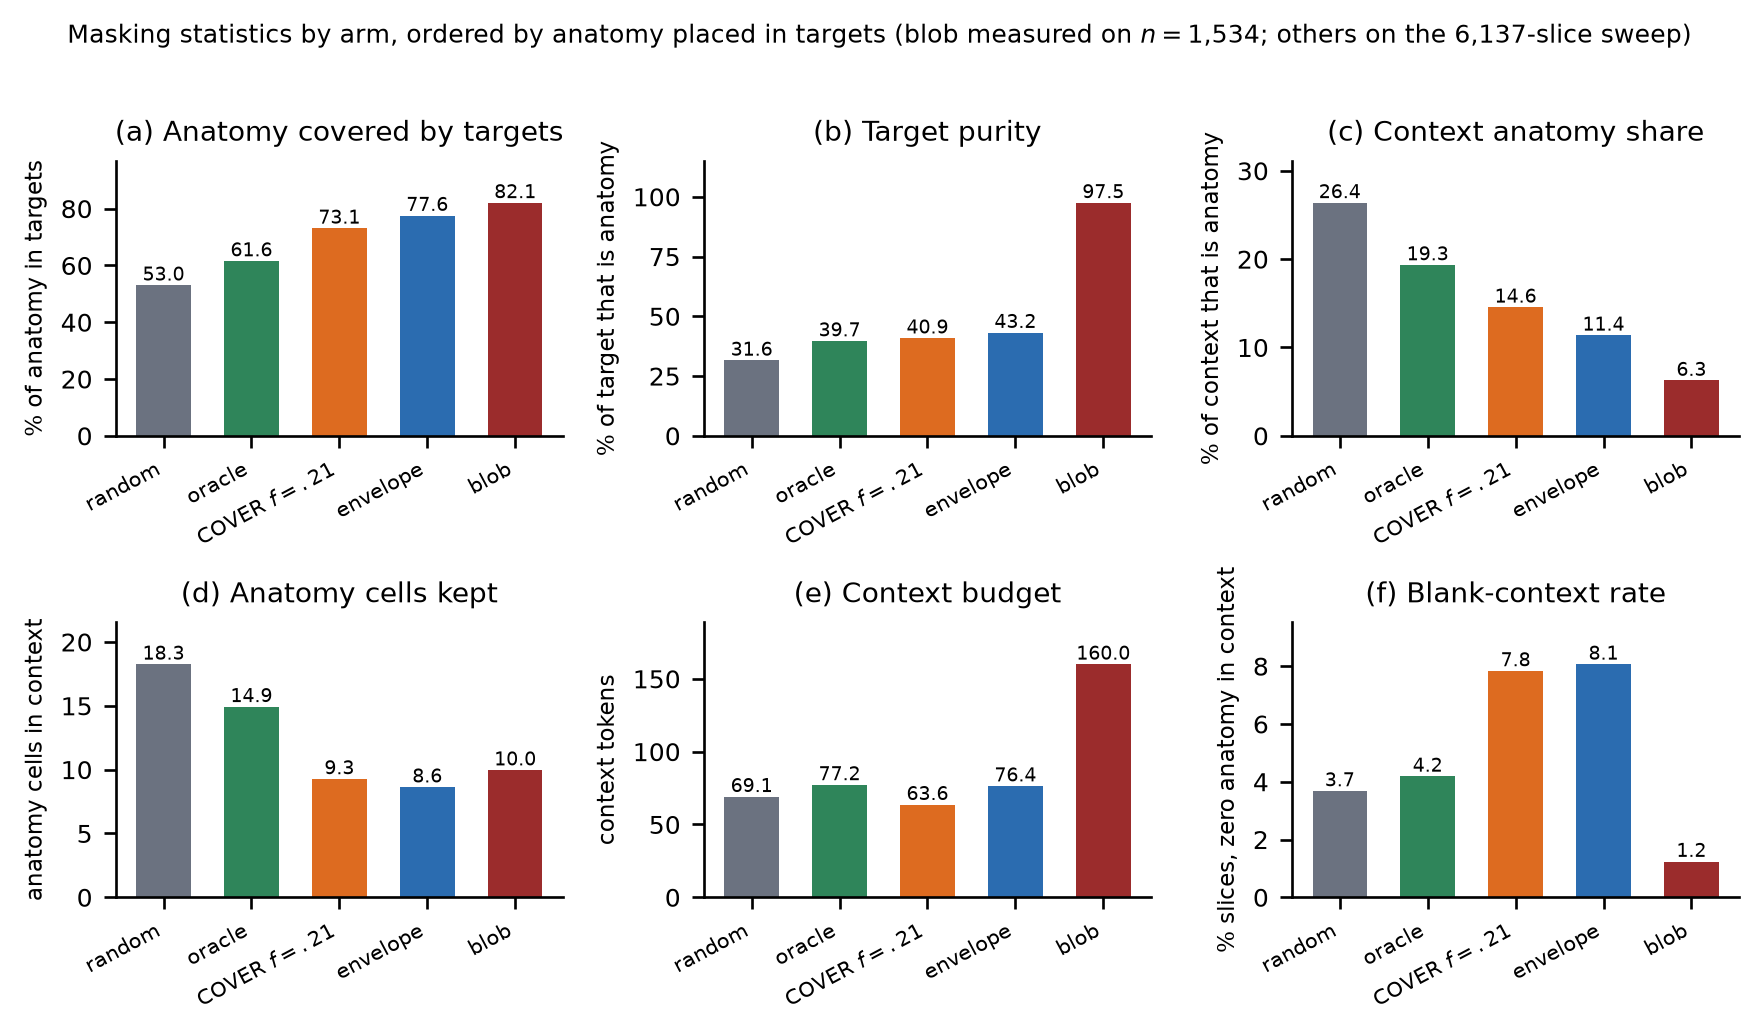
\includegraphics[width=\linewidth]{figS5_mask_statistics.png}
\caption{What each sampler actually does, measured on the 6,137-slice sweep
(\textsc{anatomy-v2} on $n{=}1{,}534$). Panel (a) is the quantity the
\textsc{cover} arm was built to maximise: it reaches $73.1\%$, \emph{below}
\textsc{envelope}'s $77.6\%$, which is the discrepancy Appendix~\ref{app:covbug}
explains. Panel (b) shows the ordering this paper tests: target purity
rises monotonically from \textsc{random} to \textsc{anatomy-v2}, while downstream
AUC does not follow it. Panels (c)--(f) give the confounds we do not
disentangle --- how much anatomy survives in the context, the context budget, and
how often a slice is left with no anatomy visible at all.}
\label{fig:maskstats}
\end{figure}

Figure~\ref{fig:policies} shows one B-scan for legibility.
Figure~\ref{fig:policies5} repeats the same rendering on five B-scans sampled
across the depth of a volume, so that the stability of each policy under
changing retinal geometry can be inspected. The samplers, the colour
assignment, and the anatomy contour are identical to Figure~\ref{fig:policies}.

\begin{figure}[p]
\centering
\includegraphics[width=\linewidth,height=0.86\textheight,keepaspectratio]%
{fig_masking_policies.png}
\caption{All six masking policies (columns) on five B-scans (rows) spanning one
volume, drawn with the production samplers. Leftmost column is the unmasked
B-scan. Each predictor target block has its own colour; the green contour is
the anatomy reference. The random, envelope, and cover arms place axis-aligned
rectangles; the anatomy arms grow cell-wise targets that follow the retinal
band and therefore change shape from slice to slice.}
\label{fig:policies5}
\end{figure}

\section{Mask-geometry provenance}
\label{app:geomprov}

Table~\ref{tab:geom} was regenerated from the production samplers rather than
carried forward from an earlier draft, and this appendix records how, together
with two facts the table itself cannot show: how much of each cell is
measurement noise, and how one configuration constant moves the correlation
quoted in Section~\ref{sec:results-h3}.

\paragraph{How the geometry was measured.} Each production sampler was run on
the same 600 FairVision \emph{Training} slices (24 volumes, 25 slices each),
one image at a time, with the \textsc{cover} visible-tissue floor at its
production value $f{=}0.21$, on the $16\times16$ patch grid, with anatomy taken
from the MIRAGE guide occupancy channel at threshold $0.25$. The measurement was
repeated with three independent draws (seeds 42, 1234 and 2026). Training slices
are not a choice: the cached anatomy guides exist for the Training split only,
so three of the five production samplers cannot be run on held-out slices at
all.

\paragraph{Cell-level agreement and seed noise.} Table~\ref{tab:geom} now carries
the regenerated values, so the question is how stable they are across draws.
18 of the 25 cells fall inside the three-seed range of the measurement, i.e.\ are
indistinguishable from a re-draw. Across the four rectangle arms the
\emph{loss slots} spread is smaller than the per-arm seed spread
(Table~\ref{tab:geomprov}), so that column's ordering carries no information and
no claim in this paper depends on it. The rank order of the arms on anatomy
hidden and on purity is identical across all three draws, which is what the
rank correlations in the main text rely on.

\begin{table}[h]
\centering
\caption{Stability of two Table~\ref{tab:geom} columns across three independent
draws of the same 600-slice measurement. ``sd'' is the standard deviation over
seeds 42, 1234 and 2026. The loss-slot differences between rectangle arms are
smaller than this noise.}
\label{tab:geomprov}
\small
\begin{tabular}{lcccc}
\toprule
 & \multicolumn{2}{c}{anatomy hidden (\%)} & \multicolumn{2}{c}{loss slots} \\
\cmidrule(lr){2-3}\cmidrule(lr){4-5}
policy & value & sd & value & sd \\
\midrule
\textsc{random}     & 53.95 & 0.71 & 159.91 & 1.15 \\
\ArmBest{}          & 62.13 & 0.64 & 158.99 & 0.43 \\
\textsc{envelope}   & 77.58 & 0.38 & 159.68 & 1.00 \\
\textsc{cover}      & 73.55 & 0.30 & 159.09 & 0.45 \\
\textsc{anatomy-v2} & 79.89 & 0.39 & 64.00  & 0.00 \\
\bottomrule
\end{tabular}
\end{table}

\paragraph{The delivered context is not the per-image context.} The ``context
kept'' column of Table~\ref{tab:geom} is per-image geometry, measured before
collation. In training, every context mask in a batch is truncated to the batch
minimum, so what the encoder actually receives at the production batch size is
smaller, and unevenly so (Table~\ref{tab:delivered}). The context confound
between the anatomy arm and the rectangle arms that
Section~\ref{sec:results-h3} declines to explain
away is consequently \emph{larger} than the printed table suggests: roughly a
doubling rather than a $1.6\times$ ratio. This strengthens the verdict that H3
is not identified by this design.

\begin{table}[h]
\centering
\caption{Visible context as a fraction of the patch grid, same 600 slices and
same seed, measured per image and as delivered to the encoder at the production
batch size of 64. The per-image column reproduces
Table~\ref{tab:geom}'s ``context kept'' to within $0.4$ points.}
\label{tab:delivered}
\small
\begin{tabular}{lcc}
\toprule
policy & per image & delivered at batch 64 \\
\midrule
\textsc{random}     & 41.9\% & 24.7\% \\
\ArmBest{}          & 45.5\% & 32.9\% \\
\textsc{envelope}   & 40.6\% & 30.7\% \\
\textsc{cover}      & 43.2\% & 30.1\% \\
\textsc{anatomy-v2} & 67.7\% & 63.5\% \\
\bottomrule
\end{tabular}
\end{table}

\paragraph{The rank correlation depends on a configuration constant.} The
$+0.80$ anatomy-hidden/AUC Spearman coefficient of
Section~\ref{sec:results-h3} is computed at the production \textsc{cover} floor
$f{=}0.21$. Re-measured on the same slices with the floor at $0.15$,
\textsc{cover} hides $79.5\%$ of anatomy instead of $73.4\%$ at the same batch
size and overtakes
\textsc{envelope}, which reorders the four rectangle arms and moves the same
coefficient to $+0.40$. A rank statistic over four arms that a single
configuration constant can move by that much is not evidence about anatomy, in
either direction, which is why Section~\ref{sec:results-h3} draws its conclusion
from the direct comparison instead.

\paragraph{What would identify target shape.} An arm that isolated target shape
would have to match \textsc{envelope} on the axes that currently differ, and
those requirements are numeric, not rhetorical. \textsc{anatomy-v2} sets four
predictor targets resampled to a fixed $K{=}16$ cells, giving exactly 64 loss
slots; matching the rectangle arms' $158$--$160$ slots at four targets requires
$K\approx40$ (inferred arithmetic on those measured values). It would also have
to deliver a mask ratio of $40$--$46\%$ of the grid rather than the $21\%$ that
the anatomy arms deliver --- roughly twice the target area, which for a
shape-following sampler means more or larger blobs and therefore changes the
very shape statistics being tested --- and it would have to pass through the
rectangle collation path, including the batch-minimum truncation above. It would
then need the same replicated continuation design and the same endpoint as
Appendix~\ref{app:replication}. We did not run it; naming its specification is
what we can offer instead.

\section{Subgroup and severity analysis}
\label{app:subgroup}

\begin{figure}[h]
\centering
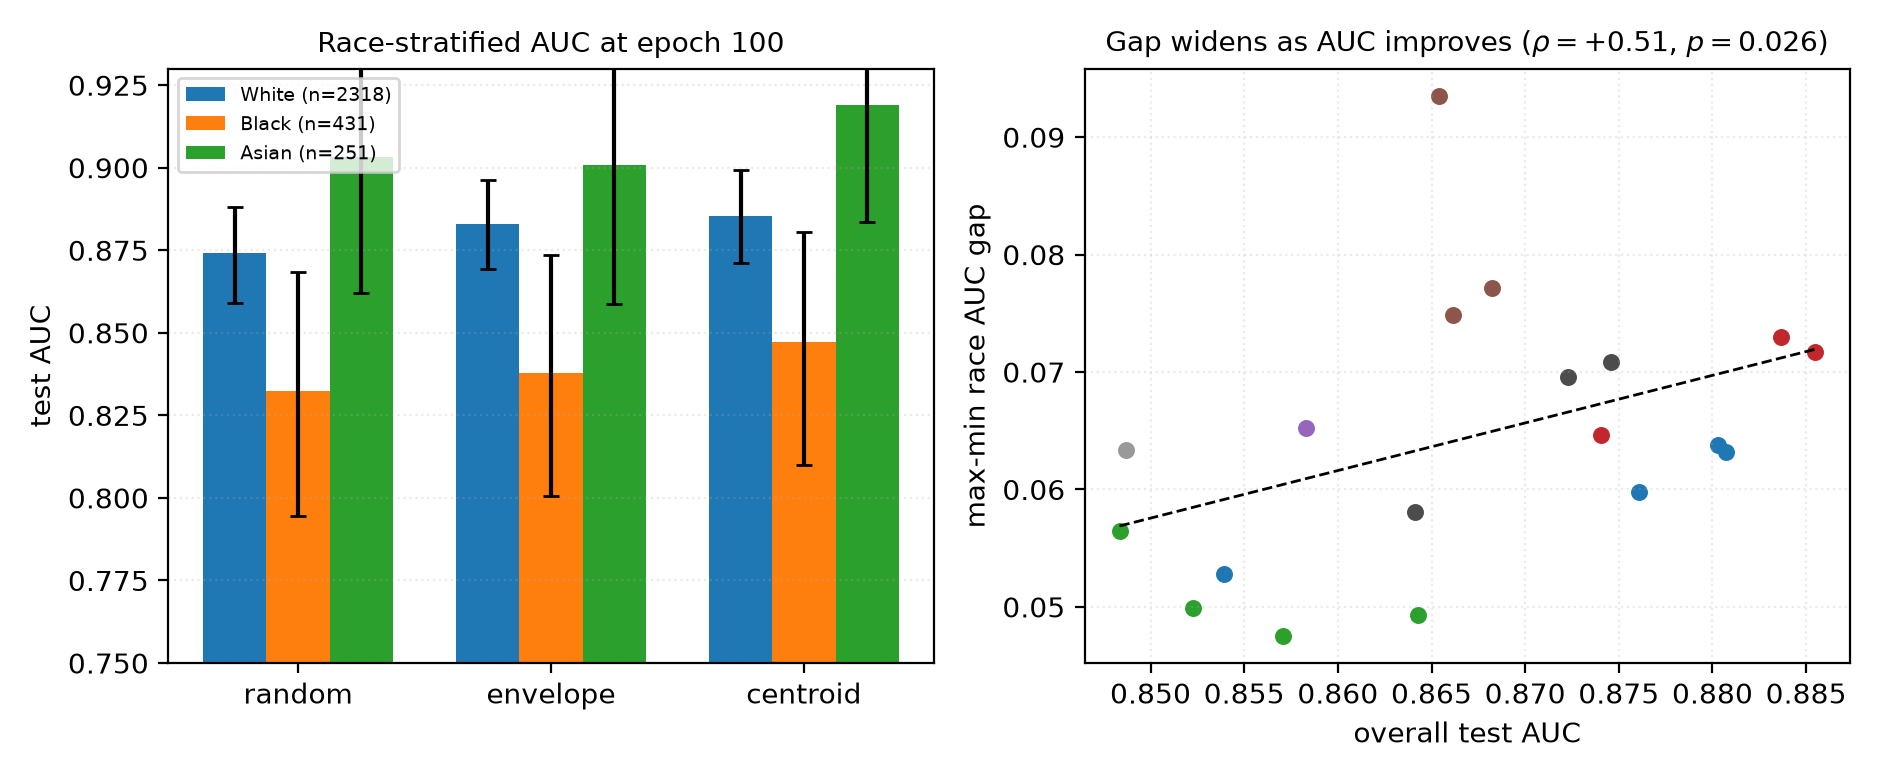
\includegraphics[width=\linewidth]{fig_fairness.png}
\caption{\textbf{Left:} race-stratified AUC at epoch 100 with bootstrap
intervals. The black subgroup is lowest under every policy, but note that
\emph{every} group improves from \textsc{random} to \ArmBest{}.
\textbf{Right:} max--min race gap against aggregate AUC across \NprobesSub{}
checkpoints. The fitted slope is positive and passes multiplicity correction at
checkpoint level, but does not survive branch-level aggregation
(Table~\ref{tab:subtrends}), so we draw no trend conclusion from it.}
\label{fig:fair}
\end{figure}

All numbers below come from saved test predictions joined to FairVision's
released metadata in deterministic loader order; the join is validated by exact
label reconstruction (\Ntest/\Ntest{} labels recovered in every probe). The
\NprobesSub{} probes used here are exactly those the inventory marks valid: the
four retracted coverage probes of Appendix~\ref{app:excluded} and the two
precision-spliced \textsc{anatomy-v2} probes are excluded here as everywhere
else in the paper.

\paragraph{Why we report two sample sizes.} The \NprobesSub{} probes span only
\NbranchesSub{} pretraining branches, because several are different epochs of
one training run. Probes within a branch share an encoder lineage, a seed and
the test split, so treating them as \NprobesSub{} independent observations is
pseudo-replication. Table~\ref{tab:subtrends} therefore reports each trend twice:
once per checkpoint, and once after averaging within each branch. Where the two
disagree, the branch-level figure is the one to believe.

\begin{table}[h]
\centering
\caption{Subgroup gap trends. ``gap range'' is the max--min subgroup AUC gap
observed across the \NprobesSub{} valid probes. $q$ is Benjamini--Hochberg
across the seven attributes tested, which is necessary because seven trends were
examined. Only sex survives correction at the conventional $0.05$ level, and it
\emph{narrows} as aggregate AUC rises. Race, ethnicity and disease severity share
the same $q$ just above that level, so no threshold admits race and severity
without also admitting ethnicity. Race is the one attribute whose
checkpoint-level trend does not
persist under branch aggregation ($p{=}0.4821$), where the effective sample is
\NbranchesSub{} independent branches rather than \NprobesSub{} probes; we
therefore draw no trend conclusion for race.}
\label{tab:subtrends}
\footnotesize
\setlength{\tabcolsep}{4pt}
\begin{tabular}{llccccccc}
\toprule
& & & \multicolumn{3}{c}{per checkpoint ($n{=}27$)} & \multicolumn{2}{c}{per branch ($n{=}11$)} \\
\cmidrule(lr){4-6}\cmidrule(lr){7-8}
attribute & worst group & gap range & $\rho$ & $p$ & $q$ & $\rho$ & $p$ \\
\midrule
sex & female (27/27) & 0.0270--0.0396 & -0.739 & $<$0.0001 & $<$0.0001 & -0.891 & 0.0002 \\
race & black (27/27) & 0.0433--0.0935 & +0.487 & 0.0100 & 0.0232 & +0.518 & 0.1025 \\
ethnicity & hispanic (27/27) & 0.0203--0.0661 & +0.151 & 0.4509 & 0.4509 & +0.409 & 0.2115 \\
language & other languages (22/27) & 0.0518--0.0805 & +0.184 & 0.3589 & 0.4187 & +0.400 & 0.2229 \\
marital status & single (27/27) & 0.0349--0.0654 & -0.380 & 0.0503 & 0.0881 & -0.373 & 0.2589 \\
age & $<$60 (26/27) & 0.0474--0.0704 & +0.300 & 0.1279 & 0.1791 & +0.236 & 0.4841 \\
disease severity & mild ($-6$,$-2$] (27/27) & 0.1266--0.1400 & -0.551 & 0.0029 & 0.0102 & -0.618 & 0.0426 \\
\bottomrule
\end{tabular}

\end{table}

\paragraph{Race.} The black subgroup has the lowest AUC in every one of the
\NprobesSub{} probes ($n{=}\NBlack$ black, $n{=}\NAsian$ asian, $n{=}\NWhite$
white; Figure~\ref{fig:fair}). At matched epoch 100 the black subgroup improves from
$\RaceRandomBlack$ under \textsc{random} to $\RaceOracleBlack$ under
\ArmBest{} ($\BlackGainOracle$), a larger absolute gain than the white
subgroup's ($\RaceRandomWhite \to \RaceOracleWhite$). The max--min gap
nonetheless widens slightly, because the asian subgroup --- already the
highest --- gains most ($\RaceRandomAsian \to \RaceOracleAsian$). A widening
max--min gap with universally rising subgroup AUCs is not evidence of harm. The
checkpoint-level correlation between aggregate
AUC and racial gap is $\rho{=}\SubRaceRho$ ($p{=}\SubRaceRhoP$). It does not
pass Benjamini--Hochberg correction at the stated conventional threshold
($q{=}\SubRaceQ$), and it vanishes once probes are aggregated to their
pretraining branches ($\rho{=}\SubRaceBranchRho$,
$p{=}\SubRaceBranchP$), and the checkpoint-level test is pseudo-replicated
because the \NprobesSub{} probes come from only \NbranchesSub{} branches.

\paragraph{Disease severity.} FairVision's label is defined by visual-field mean
deviation (md): every test volume with md $\leq -2$ is positive. Severity
therefore cannot be used as an ordinary subgroup axis, because within-bin AUC is
undefined --- a trap that silently yields nothing under naive stratification.
Instead each positive stratum is scored against the shared pool of all
\Nneg{} negatives (Table~\ref{tab:severity}).

\begin{table}[h]
\centering
\caption{Severity-stratified AUC at matched epoch 100. Each positive stratum is
scored against the shared pool of all \Nneg{} negatives. Every stratum improves;
the gains were not tested against one another.}
\label{tab:severity}
\small
\begin{tabular}{lccccc}
\toprule
stratum & $n_{+}$ & \textsc{random} & \textsc{envelope} & \ArmBest{} & $\Delta$ \\
\midrule
severe (md $\leq -12$)          & 334 & \SevRandomSevere   & \SevEnvelopeSevere   & \SevOracleSevere   & \SevDeltaSevere \\
moderate ($-12 <$ md $\leq -6$) & 460 & \SevRandomModerate & \SevEnvelopeModerate & \SevOracleModerate & \SevDeltaModerate \\
mild ($-6 <$ md $\leq -2$)      & 672 & \SevRandomMild     & \SevEnvelopeMild     & \SevOracleMild     & \textbf{\SevDeltaMild} \\
\bottomrule
\end{tabular}
\end{table}

The severe-to-mild gap is $\SevGapRandom$ for the null and $\SevGapOracle$ for
the strongest policy, and stays within $\SeverityGapSpread$
($\SubSeverityGapMin$--$\SubSeverityGapMax$) across all \NprobesSub{} probes
while aggregate AUC spans $\SubAUCMin$--$\SubAUCMax$. Target placement raises
the whole severity curve, all three strata separated from zero under paired
resampling (Table~\ref{tab:pairedsub}), the largest point estimate at mild
disease ($\PDSevMildDelta$, CI
$\PDSevMildCI$) and the smallest at severe ($\PDSevSevereDelta$). That ordering
is descriptive only: we did not test the paired \emph{difference} between
strata, so it does not establish that mild disease benefits most. We note that
mild functional loss is harder to separate from normal OCT by construction, so
the difficulty ordering is expected clinically; what the data add is that no
masking policy we tested changes it.

\begin{table}[h]
\centering
\caption{Paired change in subgroup AUC from \textsc{random} to
\ArmBest{} at matched epoch 100. Each bootstrap draw resamples subjects
once and applies the same resampled set to both arms and every stratum, so these
are paired differences rather than differences of independent estimates.}
\label{tab:pairedsub}
\small
\begin{tabular}{lcccc}
\toprule
stratum & $n$ & $\Delta$ AUC & 95\% CI & excludes 0 \\
\midrule
severity, mild & 2206 & +0.01372 & [+0.00541,\,+0.02192] & yes \\
severity, moderate & 1994 & +0.01016 & [+0.00262,\,+0.01757] & yes \\
severity, severe & 1868 & +0.00626 & [+0.00104,\,+0.01187] & yes \\
race, White & 2318 & +0.01129 & [+0.00518,\,+0.01731] & yes \\
race, Black & 431 & +0.01467 & [-0.00055,\,+0.03060] & no \\
race, Asian & 251 & +0.01558 & [-0.00079,\,+0.03283] & no \\
sex, Female & 1716 & +0.01152 & [+0.00412,\,+0.01890] & yes \\
sex, Male & 1284 & +0.01006 & [+0.00335,\,+0.01678] & yes \\
\bottomrule
\end{tabular}

\end{table}

\paragraph{Limitations.} The $p$-values here are descriptive, for the reasons
given in Section~\ref{sec:limits}. Race and ethnicity are
self-reported categories inherited from FairVision's coding. A race-by-sex
intersectional breakdown \emph{is} reported, in
Appendix~\ref{app:intersectional}; its limits are that two of its six cells hold
fewer than $130$ cases and that it carries no paired per-cell intervals, so it
describes the disparity and tests no per-cell change.
All figures are frozen mean-pool
linear probes. Subgroup sensitivity at a transferred threshold is reported in
Appendix~\ref{app:operating}, but we report no subgroup calibration and no
subgroup predictive values, so this is not a complete fairness
evaluation. Disparities
could differ under fine-tuning or a stronger head.

\subsection{Intersectional breakdown: race by sex}
\label{app:intersectional}

The audit above crosses no attributes, so on its own it cannot say whether a
group disadvantaged on two axes at once is worse served than either margin
implies. We therefore also computed AUC for all six race-by-sex cells of the
test split, from the same saved predictions, under the same exact-label join
proof, with per-arm bootstrap percentile intervals from the same helper as the
marginal audit. The second axis is FairVision's self-reported gender coding,
which this paper reports as sex throughout. The artifact behind this subsection
covers 22 arms, 18 of them non-retracted; those 18 are a strict subset of the
\NprobesSub{} probes of Table~\ref{tab:subtrends} --- five \textsc{cover} and
\textsc{blob} probes are absent from it --- so every count in this subsection is
out of 18 arms, not \NprobesSub{}.

\begin{table}[h]
\centering
\caption{Race-by-sex AUC at matched epoch 100 on the \Ntest{} test volumes, with
per-cell counts and per-arm bootstrap percentile intervals. $\Delta$ is
\ArmBest{} minus \textsc{random} as a difference of point estimates. The
artifact stores per-arm intervals only and no paired per-cell resampling, so no
$\Delta$ in this table is tested against zero; per-cell significance is PENDING.
The two asian cells are small ($n{=}123$ and $n{=}128$) and their intervals are
correspondingly wide.}
\label{tab:intersectional}
\scriptsize
\setlength{\tabcolsep}{3.5pt}
\begin{tabular}{lrrcccr}
\toprule
cell & $n$ & $n_{+}$ & \textsc{random} & \textsc{envelope} & \ArmBest{} & $\Delta$ \\
\midrule
asian $\times$ female & 123  & 52  & 0.8761 [0.8024, 0.9342] & 0.8762 [0.8042, 0.9366] & 0.8904 [0.8245, 0.9423] & $+0.0144$ \\
asian $\times$ male   & 128  & 66  & 0.9245 [0.8752, 0.9655] & 0.9145 [0.8565, 0.9626] & 0.9409 [0.8983, 0.9751] & $+0.0164$ \\
black $\times$ female & 250  & 149 & 0.8195 [0.7668, 0.8679] & 0.8155 [0.7632, 0.8638] & 0.8309 [0.7790, 0.8783] & $+0.0114$ \\
black $\times$ male   & 181  & 119 & 0.8435 [0.7822, 0.8994] & 0.8652 [0.8091, 0.9141] & 0.8663 [0.8132, 0.9149] & $+0.0228$ \\
white $\times$ female & 1343 & 610 & 0.8641 [0.8441, 0.8826] & 0.8728 [0.8530, 0.8910] & 0.8762 [0.8570, 0.8943] & $+0.0121$ \\
white $\times$ male   & 975  & 470 & 0.8864 [0.8650, 0.9062] & 0.8958 [0.8744, 0.9148] & 0.8962 [0.8746, 0.9153] & $+0.0099$ \\
\midrule
max$-$min gap         &      &     & 0.1050 & 0.0990 & 0.1100 & \\
\bottomrule
\end{tabular}
\end{table}

\paragraph{The ordering compounds, and it never reorders.} The black
$\times$ female cell has the lowest AUC in all 18 non-retracted arms and the
asian $\times$ male cell the highest in all 18. Within each race the female cell
sits below the male cell in all $54$ race-by-arm combinations, and within each
sex the black cell sits below the white cell in all $36$. These 18 arms share one
test split, one epoch-25 ancestor and one probe seed, and several are different
epochs of a single branch, so this unanimity is a consistency check across
checkpoints, not 18 replications; we attach no $p$-value to it, exactly as for
the marginal ordering above.

\paragraph{The marginal race gap understates the worst cell.} Averaged over the
18 arms, the max$-$min gap is $0.0340$ by sex alone, $0.0653$ by race alone, and
$0.1046$ across the six race-by-sex cells, and the intersectional gap exceeds
that arm's marginal race gap in all 18. The race margin therefore understates
the spread a race-by-sex reading exposes by $60.1\%$ on average --- arithmetic on
those two means, not a separate measurement. The same pattern holds at the
matched epoch of Table~\ref{tab:intersectional}: under \ArmBest{} the marginal
race gap is $0.0717$ while the race-by-sex gap is $0.1100$, and the worst cell,
black $\times$ female at $0.8309$, sits $0.0163$ below the marginal black figure
$\RaceOracleBlack$ that the marginal audit above reports. An audit that stops
at the margins reports a worst-group number that is optimistic relative to the
worst cell. The compounding is close to additive and we do not claim more: the
sex and race means sum to $0.0993$ against an observed $0.1046$, a ratio of
$1.053$, which is not evidence of a super-additive interaction.

\paragraph{Not every cell improves.} The statement elsewhere in this appendix
that every subgroup point estimate rises from \textsc{random} to \ArmBest{} is a
statement about marginal strata at the matched epoch, and it does \emph{not}
extend to cells at every epoch. At epoch 100 all six cells do rise
(Table~\ref{tab:intersectional}), but at epoch 50 the asian $\times$ female cell
falls by $0.0020$, and \textsc{envelope} minus \textsc{random} is negative in
three of six cells at epoch 75 (asian $\times$ female $-0.0148$, asian $\times$
male $-0.0031$, black $\times$ female $-0.0025$) and in two of six at epoch 100
(asian $\times$ male $-0.0100$, black $\times$ female $-0.0040$, with asian
$\times$ female at $+0.0001$). No policy we tested raises every intersectional
cell at every epoch, and the exceptions fall in the small asian cells and in the
worst cell.

\paragraph{What this does not establish.} There are no paired per-cell bootstrap
intervals in the artifact, so every $\Delta$ above is a difference of point
estimates and none of them is separated from zero; per-cell delta significance
is PENDING and is computable from the retained per-arm predictions. Two cells
carry $n{=}123$ and $n{=}128$, so their intervals overlap almost everything.
Cells with a single class or fewer than $40$ cases would have been dropped; none
were, so all six race-by-sex cells are reported. Nothing here is a fairness
intervention: as with the margins, no policy reorders the cells, and the
worst-served cell is the same under the unguided null and under every guided
policy we tested.

\section{Excluded runs}
\label{app:excluded}

Four probes of an earlier \emph{null} run are excluded from all analysis. They
are unguided-masking controls from a superseded coverage campaign --- the
inventory lists them under \textsc{random}, and their run tags begin
\texttt{frozen\_cover\_random} because of that campaign, not because they use a
coverage policy. They were
trained with half-precision EMA targets and a different encoder-truncation
policy from the arms they would be compared against, so their deficit is not
attributable to masking. Similarly, the \textsc{anatomy-v2} probes at
epochs 75 and 92 follow a change of target precision partway through that arm's
training; they are listed in Table~\ref{tab:allprobes} but excluded from the
matched-epoch comparisons in Table~\ref{tab:main}.

\section{A collation defect in the coverage arm, and what it invalidates}
\label{app:covbug}

We audited the \textsc{cover} sampler after its epoch-100 result and found a
defect. It invalidates the reading of that arm and weakens one cross-family
comparison.

\paragraph{The defect.} Predictor targets are collated by truncating every target
to the length of the shortest target anywhere in the microbatch. \textsc{cover}
chooses its placement \emph{before} this happens: it greedily maximises hidden
anatomy subject to a visible-tissue floor, evaluated on full rectangles, and the
collator then shortens those rectangles. The optimisation is therefore defeated
after the fact.

\paragraph{Measured consequences.} A one-off audit found that collation reduced
\textsc{cover}'s anatomy coverage; an independent sweep over $6{,}137$ slices
gives $73.1\%$ against $77.6\%$ for \textsc{envelope}. The arm intended to hide
\emph{more} anatomy than \textsc{envelope} in fact hides \emph{less}. Across
$24{,}000$ emitted targets only $73.4\%$ remain perfect
rectangles. Because target cells are enumerated row-major, truncation keeps the
top of each rectangle and discards the bottom, so the loss is directional rather
than a neutral shrink. \emph{Provenance:} the one-off CPU audit of 194 accepted
slices that first exposed the defect was not persisted, so its pre- and
post-truncation figures are no longer asserted. The $73.1\%$ against $77.6\%$
comparison, which is the only figure the body relies on, is backed by the stored
floor sweep and is unaffected.

\paragraph{Why it went unnoticed.} Realised coverage is recorded before
truncation. Every training log therefore reported the intended figure, and the
instrument agreed with the design rather than with the data.

\paragraph{What it invalidates.} We cannot claim that \textsc{cover} tests
aggressive anatomy coverage, nor that its decline shows over-covering anatomy is
harmful; on delivered masks it does not out-cover \textsc{envelope}. Its measured
trajectory remains a real property of the policy as implemented. The mask
geometry in Table~\ref{tab:geom} is unaffected, having been measured on delivered
masks.

\paragraph{Scope.} \textsc{envelope} shares the same collation path and the same
directional clipping, but sets no exact coverage target, so it has no comparable
optimisation to defeat. The anatomy arms instead resample every target to a fixed
$K{=}16$ cells. Contrasts within the rectangle family are collated identically
and are unaffected; the anatomy-versus-rectangle contrast is not, and we treat it
accordingly in Section~\ref{sec:results}. A corrected coverage arm must be
retrained from the shared ancestor, since patching mid-trajectory would splice
two masking policies into one curve.

\paragraph{Status of a corrected run.} At submission the corrected arm is
\CoverFixedStatus{}. Until it exists, the question this arm was built to answer
--- whether hiding most of the anatomy is harmful --- remains \emph{open}.

\section{Why unguided masking is such a strong baseline}
\label{app:bg}

Unguided masking spends most of its predictor targets on background, yet it
reaches within $\DOracleRandomEpHundred$ of the best policy. We investigated
whether background carries diagnostic signal, and whether position embeddings are
the mechanism.

\paragraph{Background is a real \emph{pretraining} signal.} At epoch 100 the
random arm's predictor beats a per-position, no-context reference by $0.680$ on
background targets, above its $0.633$ on anatomy targets: predicting a background
token requires more than knowing where it is. Pretraining also spends capacity
reorganising background --- background self-similarity falls from $0.784$
untrained to $0.346$ at epoch 100.

\paragraph{But it does not help the classifier.} Pooled background features are
$95.2\%$ linearly reconstructible from pooled anatomy features. Residualised,
background predicts glaucoma at test AUC $0.5515$ (CI $[0.5165, 0.5893]$).
Appending background to anatomy \emph{lowers} test AUC by $0.0076$
(CI $[-0.0139, -0.0012]$) for the random arm and moves it under $\pm0.002$ for
every other. A background-only probe scores $0.867$; self-attention mixes tissue
information into background tokens, so that figure cannot be read as background
signal, and we did not measure how much mixing occurs.

\paragraph{Position dominates background tokens, but is not the whole story.} At
layer 0, $90.8\%$ of the across-position variance of the encoder input at
background cells comes from \texttt{pos\_embed}, against $40.8\%$ at tissue cells
(stable across six thresholds and both checkpoints). Mechanically a background
token is close to its position code. That the predictor still beats a
per-position reference shows the pretraining signal is not purely positional.
The causal chain from this mechanism to downstream AUC remains open.

\paragraph{The two controls that would settle it, neither of which was run.}
First, a regional probe on an \emph{eroded} background region --- background
cells at a fixed minimum distance from any tissue cell --- which removes the
tokens most exposed to local mixing while keeping the probe protocol fixed.
Second, a background-content shuffle in which background token \emph{contents}
are permuted across images while positions and token count are held fixed: if
the background-only AUC survives that, the signal is positional rather than
content-bearing. Both are PENDING; neither has been run, so this appendix
reports a mechanism that is described but not established.

\section{Label efficiency}
\label{app:labeleff}

We measured each policy as supervision is withdrawn
(Section~\ref{sec:labeleff}). We
subsample the labelled training set to fractions of its size, fit the same frozen
linear probe on cached epoch-\LEEpoch{} features, and repeat \LERepeats{} times
per fraction. The per-fraction seed depends only on fraction and repeat, never on
arm, so all arms see identical label subsets and the comparison is paired.

\paragraph{Protocol parity.} This sweep uses the \emph{same} probe protocol as
Table~\ref{tab:main} --- minibatches of 256, AdamW at $4{\times}10^{-4}$, weight
decay 0.05, 50 epochs with 5 warmup and cosine decay, and the epoch selected on
validation AUC. An earlier cheaper full-batch fit disagreed with the primary
protocol. Under matched protocols, restricting this check to the null and
\ArmBest{}, their full-supervision results agree to within $0.0003$
($\LERandomHundred$ against $\AUCRandomEpHundred$ for the null,
$\LEOracleHundred$ against $\AUCOracleEpHundred$ for \ArmBest{}), so the curve
below and the headline table describe one probe, not two. This two-arm bound is
distinct from the four-arm bound reported in Section~\ref{sec:labeleff}.

The advantage of guided masking is concentrated where labels are scarce
(Table~\ref{tab:labeleff}, Figure~\ref{fig:labeleff}).
At $5\%$ of labels ($n{=}\LENFive$) \ArmBest{} leads the null by $\LEGapFive$
($\LEOracleFive$ against $\LERandomFive$), against $\LEGapHundred$ at full
supervision --- more than four times the margin. At $1\%$ the gap is wider still
($\LEOracleOne$ against $\LERandomOne$), though the standard deviations there
($\LESDRandomOne$--$\LESDCoverOne$ across arms) are large enough that we read the
ordering but not its precise size.

The defective \textsc{cover} arm (Appendix~\ref{app:covbug}) is the worst arm at
every fraction, reaching only $\LECoverOne$ at $1\%$ against $\LERandomOne$ for
the null, consistent with its targets being degraded rather than merely
differently placed.

\begin{table}[h]
\centering
\caption{Label efficiency: frozen-probe test AUC against the fraction of the
labelled training set used. All values measured, \LERepeats{} repeats per
fraction except at full data, which is deterministic.}
\label{tab:labeleff}
\small
\begin{tabular}{llcccc}
\toprule
labels & $n$ & \textsc{random} & \ArmBest{} & \textsc{envelope} & \textsc{cover} \\
\midrule
1\% & 60 & 0.7264 & 0.7436 & 0.7429 & 0.6800 \\
5\% & 300 & 0.7925 & 0.8108 & 0.8080 & 0.7768 \\
10\% & 600 & 0.8198 & 0.8166 & 0.8184 & 0.8124 \\
25\% & 1500 & 0.8533 & 0.8605 & 0.8523 & 0.8546 \\
100\% & 6000 & 0.8811 & 0.8850 & 0.8807 & 0.8785 \\
\bottomrule
\end{tabular}

\end{table}

\begin{figure}[h]
\centering
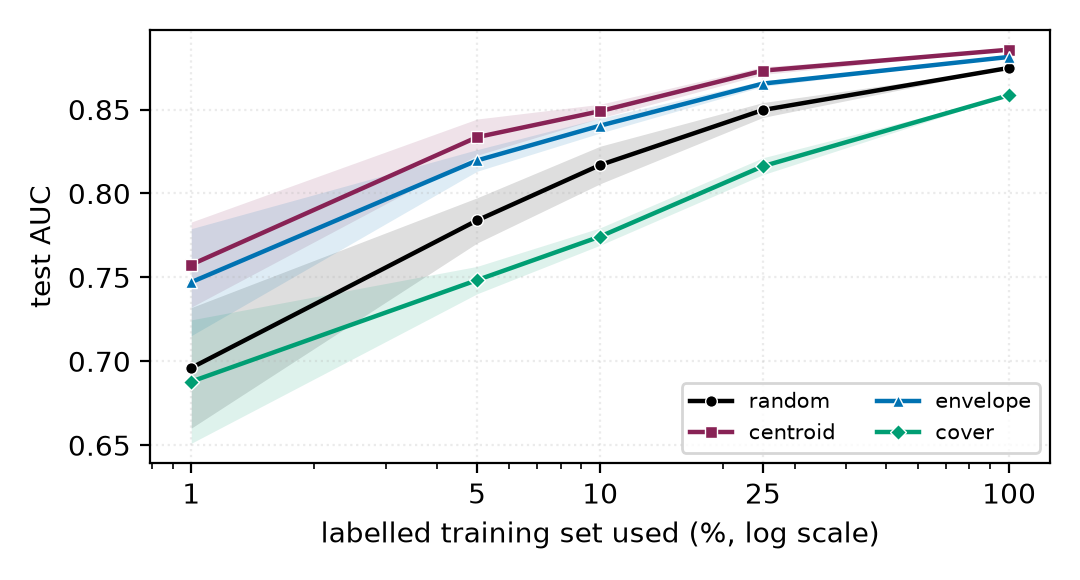
\includegraphics[width=0.60\linewidth]{fig_labeleff.png}
\caption{The policies converge as labels are added and separate as they are
removed. Shading is one standard deviation over \LERepeats{} label subsets, with
every arm seeing identical subsets. At full supervision the four arms lie within
$0.027$ of one another; at $5\%$ the spread is $0.085$.}
\label{fig:labeleff}
\end{figure}

\section{Occlusion attribution: where the classifier looks}
\label{app:interp}

The analyses in this appendix were run on the three \emph{fine-tuned} probes
(mean-pool, cross-attention pool, and a depth-1 attentive probe) that tie at test
AUC $\approx 0.887$, not on the frozen probes used for the arm comparison in the
main text. They characterise what the downstream classifier uses, and they are
reported here because two of the findings are cautionary rather than positive.
Every number in this appendix is computed from archived per-volume attribution
arrays that are not part of the released artifact set, so unlike the rest of the
paper these values cannot be recomputed from the release; only the
diffuse-attribution result at the end of the appendix is cited by the main text.

\paragraph{Method.} Attribution is by \emph{occlusion}, which is
architecture-agnostic and interventional on the model. It measures the model's
sensitivity to deleting a token, not a causal effect of anatomy on disease.
Gradient$\times$input is not used because two of
the three probes are non-linear in the slice-token matrix, where gradient
attribution is misleading. For slice-level attribution each slice token is zeroed
in turn and $\Delta$logit recorded (Figure~\ref{fig:interp-slice}); for
window-level, seven consecutive slices (Figure~\ref{fig:interp-window}); for
patch-level, leave-one-out over the 256 patch tokens of a target slice.

\begin{figure}[h]
\centering
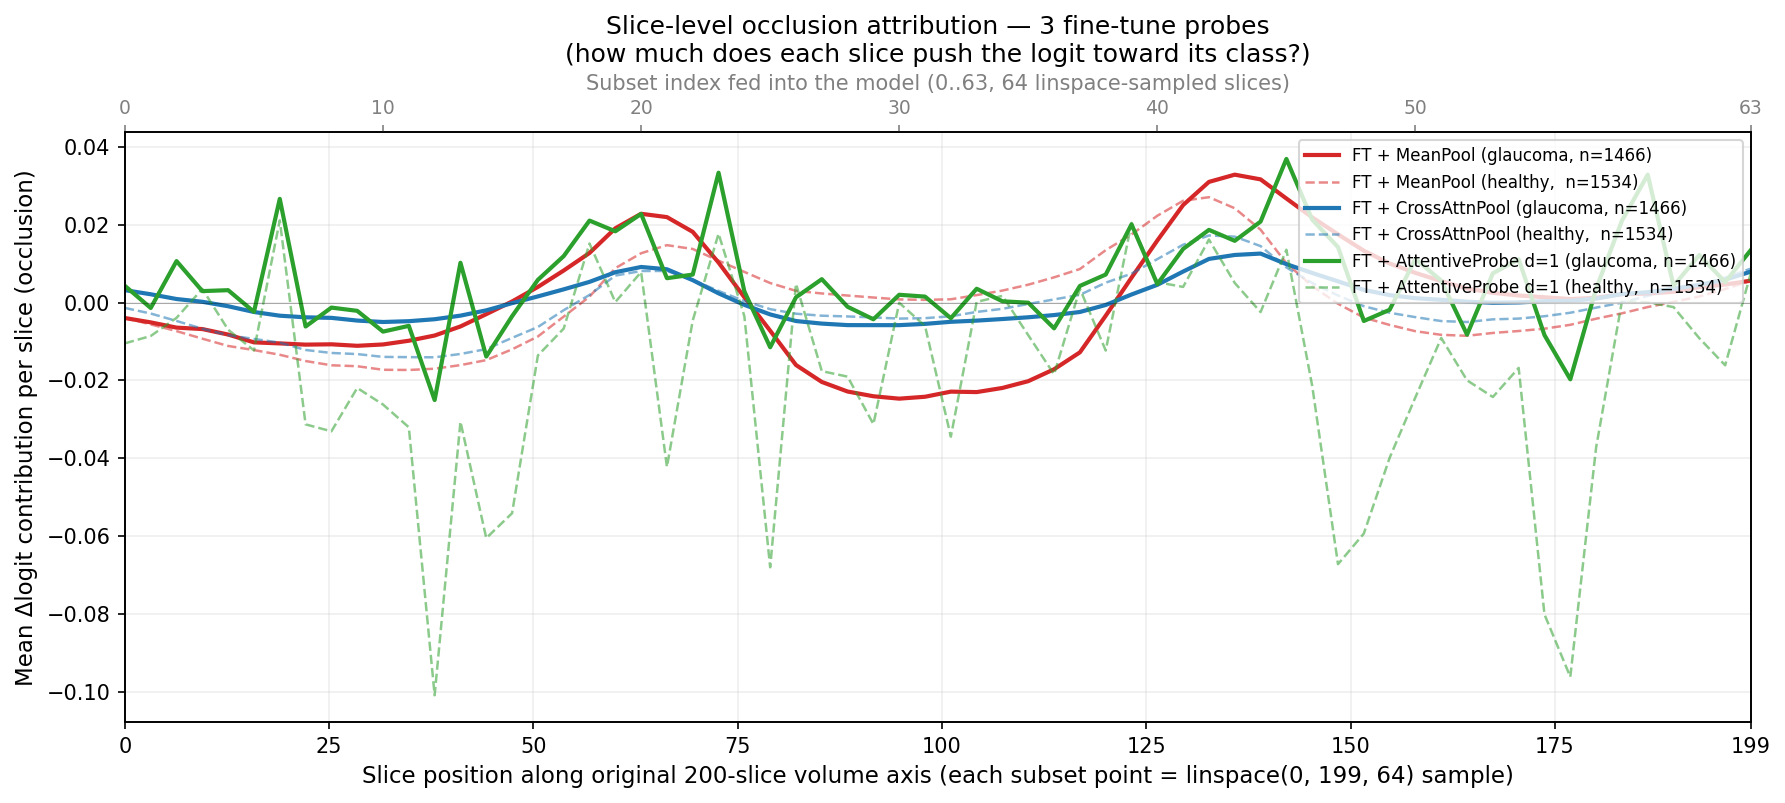
\includegraphics[width=0.92\linewidth]{interp_slice_contribution_curves.png}
\caption{Single-slice occlusion attribution against native slice position,
averaged over all \Ntest{} test volumes, for all three fine-tuned probes.
Despite spanning zero to 7.14M probe parameters they converge on the same
structure. The $y$-axis is
\emph{signed} $\Delta$logit: peaks are slices whose removal lowers the logit,
the central dip is slices whose removal raises it, and only slices near zero are
genuinely unused.}
\label{fig:interp-slice}
\end{figure}

\begin{figure}[h]
\centering
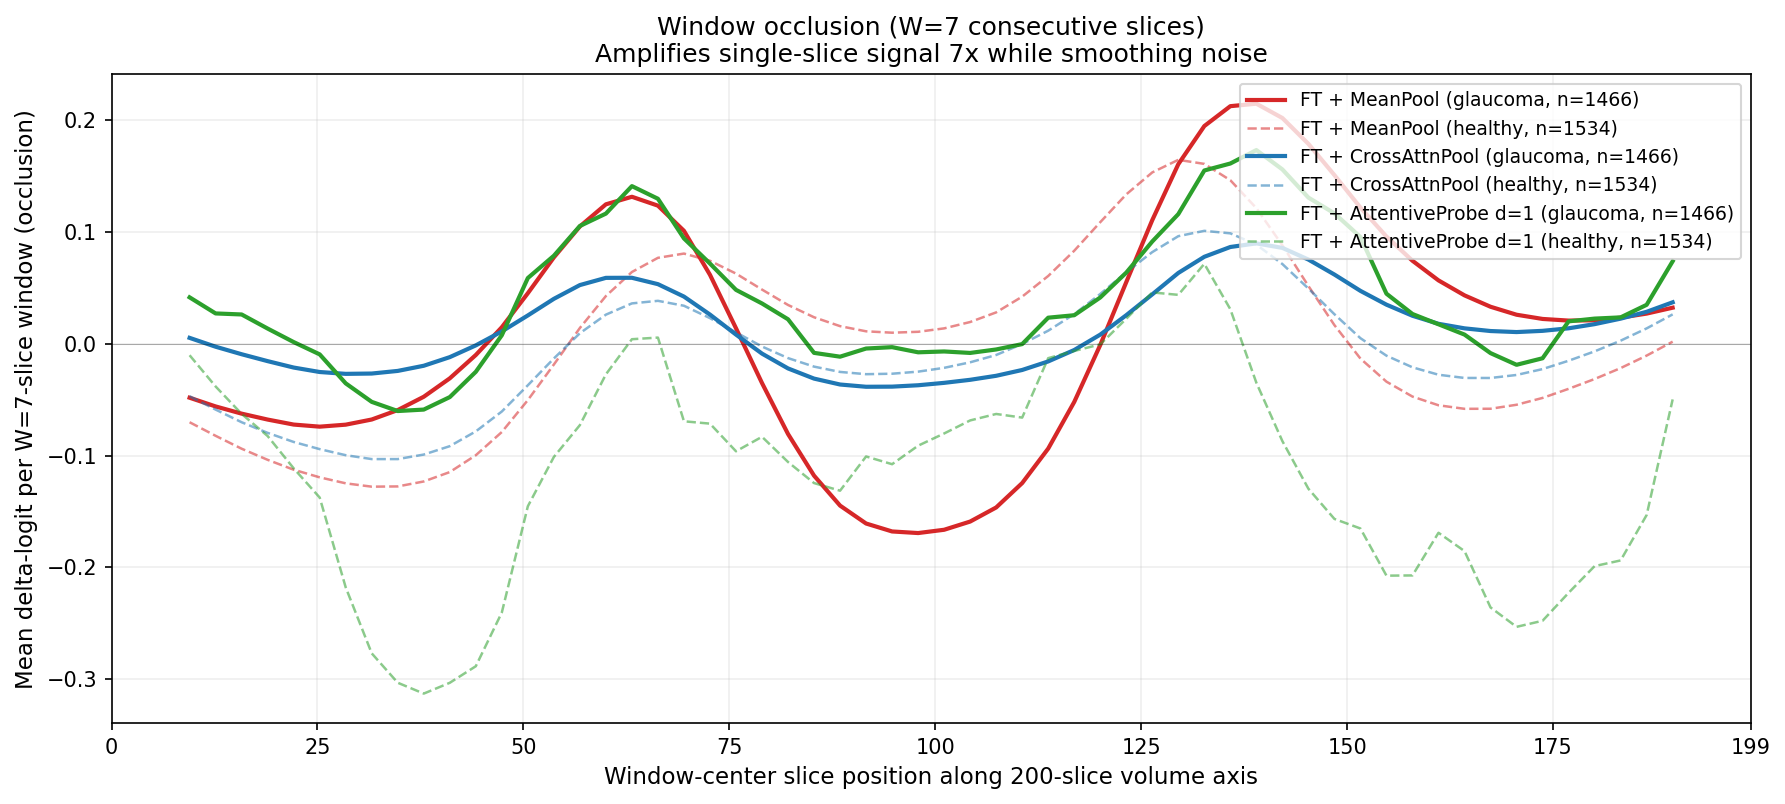
\includegraphics[width=0.92\linewidth]{interp_04_window_occlusion_W7.png}
\caption{Window occlusion ($W{=}7$) amplifies the same signal roughly sevenfold
and suppresses single-volume noise. For mean-pooled models, single-slice
occlusion systematically under-estimates attributed signal; the windowed variant
recovers more signal.}
\label{fig:interp-window}
\end{figure}

\paragraph{A bimodal attribution curve that is an artefact, not anatomy.}
The population-averaged curve is bimodal with a central dip. The tempting
reading --- that the model has
discovered the superior and inferior optic disc rim --- is \textbf{wrong}, and we
report it because it is exactly the kind of claim a plausible-looking attribution
figure invites. Three tests reject it. First, if the two peaks were bilateral
anatomy then within a diseased eye they should co-occur, giving positive
per-volume correlation between them; the peak contributions are not positively
correlated across volumes. Second,
clustering the per-volume curves into two groups yields clusters that are
near-perfect \emph{mirror images} along the slice axis for the two
well-structured probes.
Third, using that cluster label as pseudo-laterality and flipping one cluster
collapses the bimodality asymmetrically (Figure~\ref{fig:interp-odos}). What
these three tests support is an orientation or storage mixture consistent with
OD/OS: each eye carries its dominant signal on one side of the disc, the two
groups are stored with opposite axial orientation, and population averaging
manufactures an illusion of symmetry. The released metadata carries no
eye-laterality label, so the OD/OS reading is inferred from the mirror structure
and is not validated against ground truth.

\begin{figure}[h]
\centering
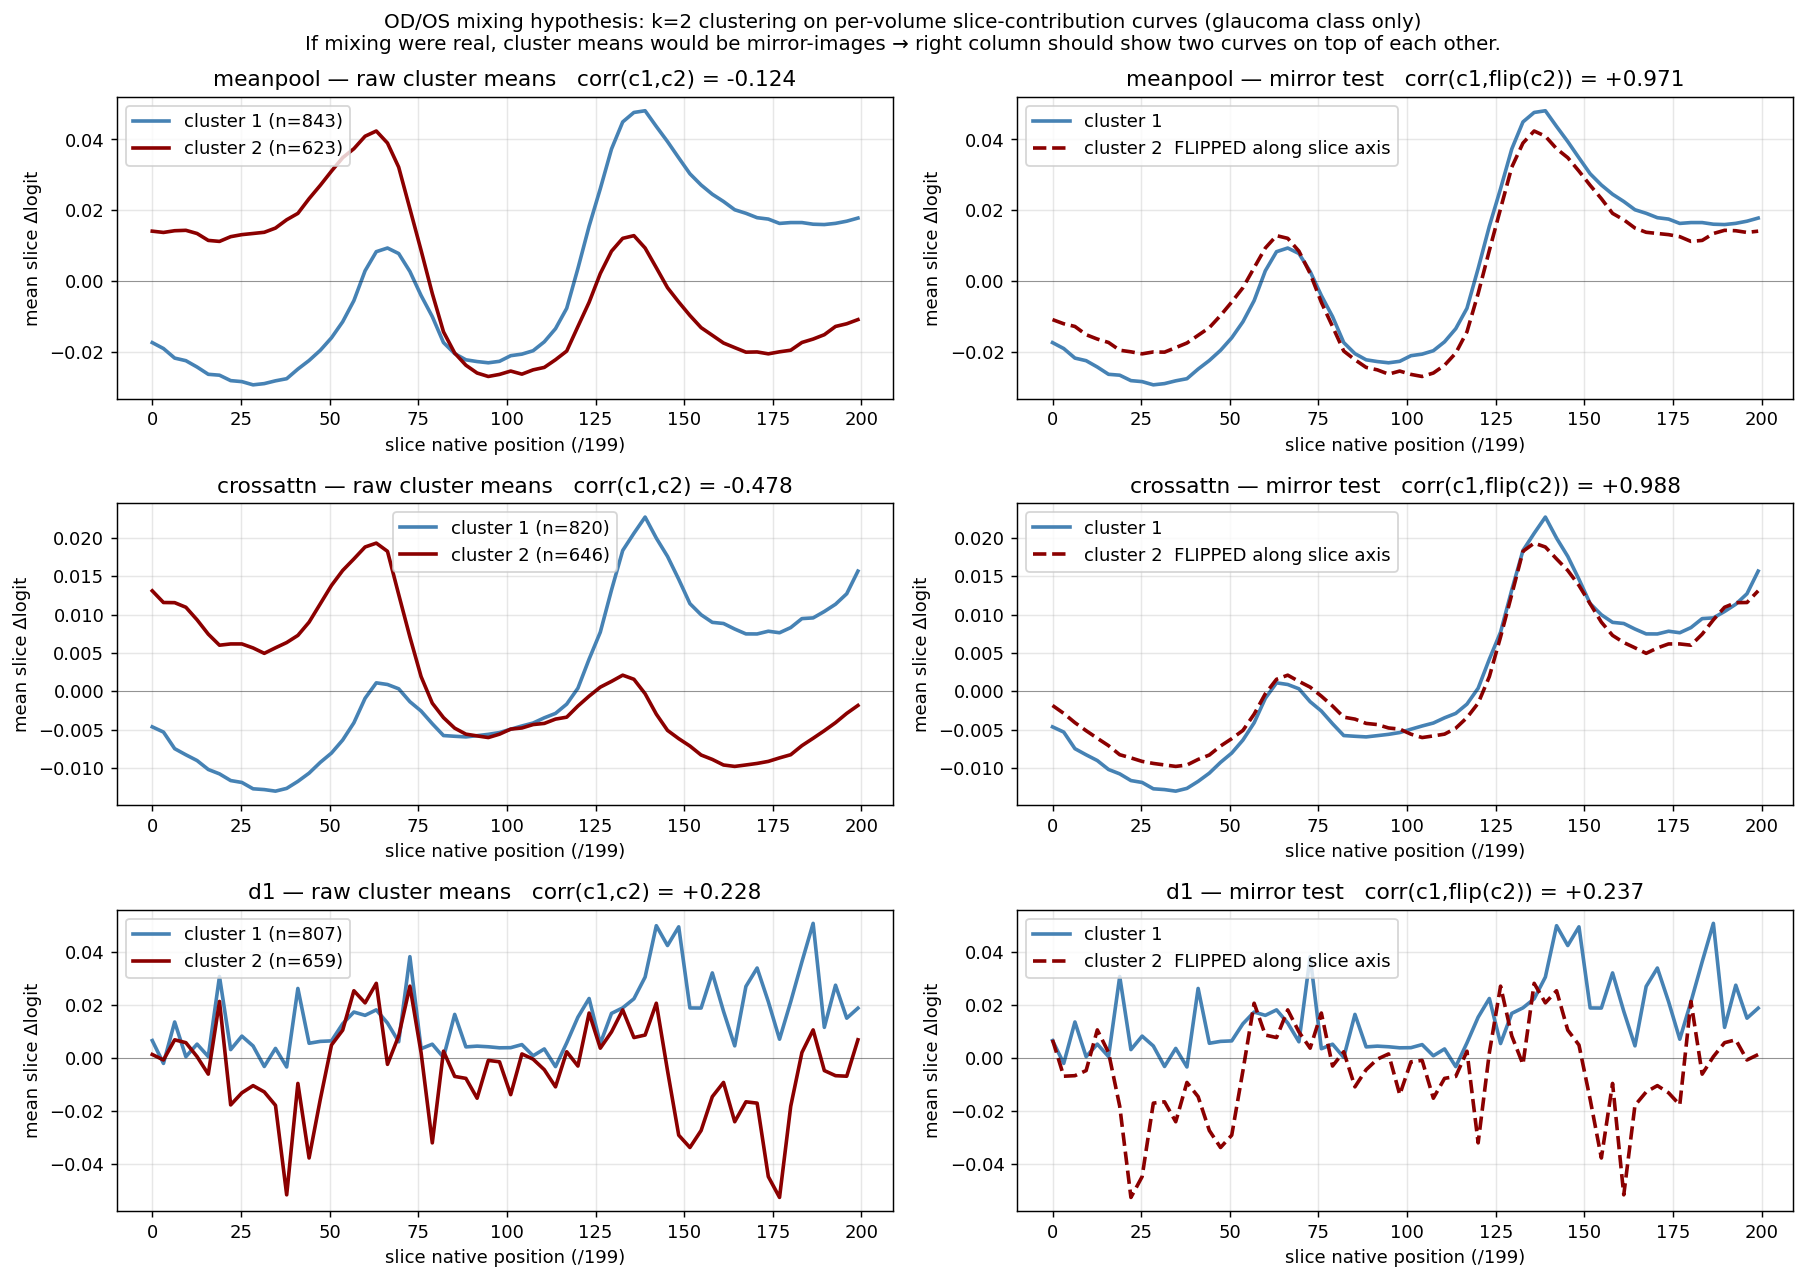
\includegraphics[width=0.92\linewidth]{interp_14_odos_mirror_test.png}
\caption{The two-peak structure is an OD/OS storage artefact. Clustering
per-volume attribution curves into two groups returns near-perfect mirror images
of one another, which is what laterality flipping would produce, rather than
bilateral anatomy.}
\label{fig:interp-odos}
\end{figure}

\paragraph{Errors are weaker signal, not different anatomy.} Stratifying by
outcome, false-negative curves are scaled-down true-positive curves with the same
shape, and false positives likewise mirror true negatives
(Figure~\ref{fig:interp-outcome}). Attribution structure
is also near-invariant to prediction confidence. The error rate at threshold $0.5$
therefore reflects signal-strength saturation on hard cases, not the model
attending to the wrong structures.

\begin{figure}[h]
\centering
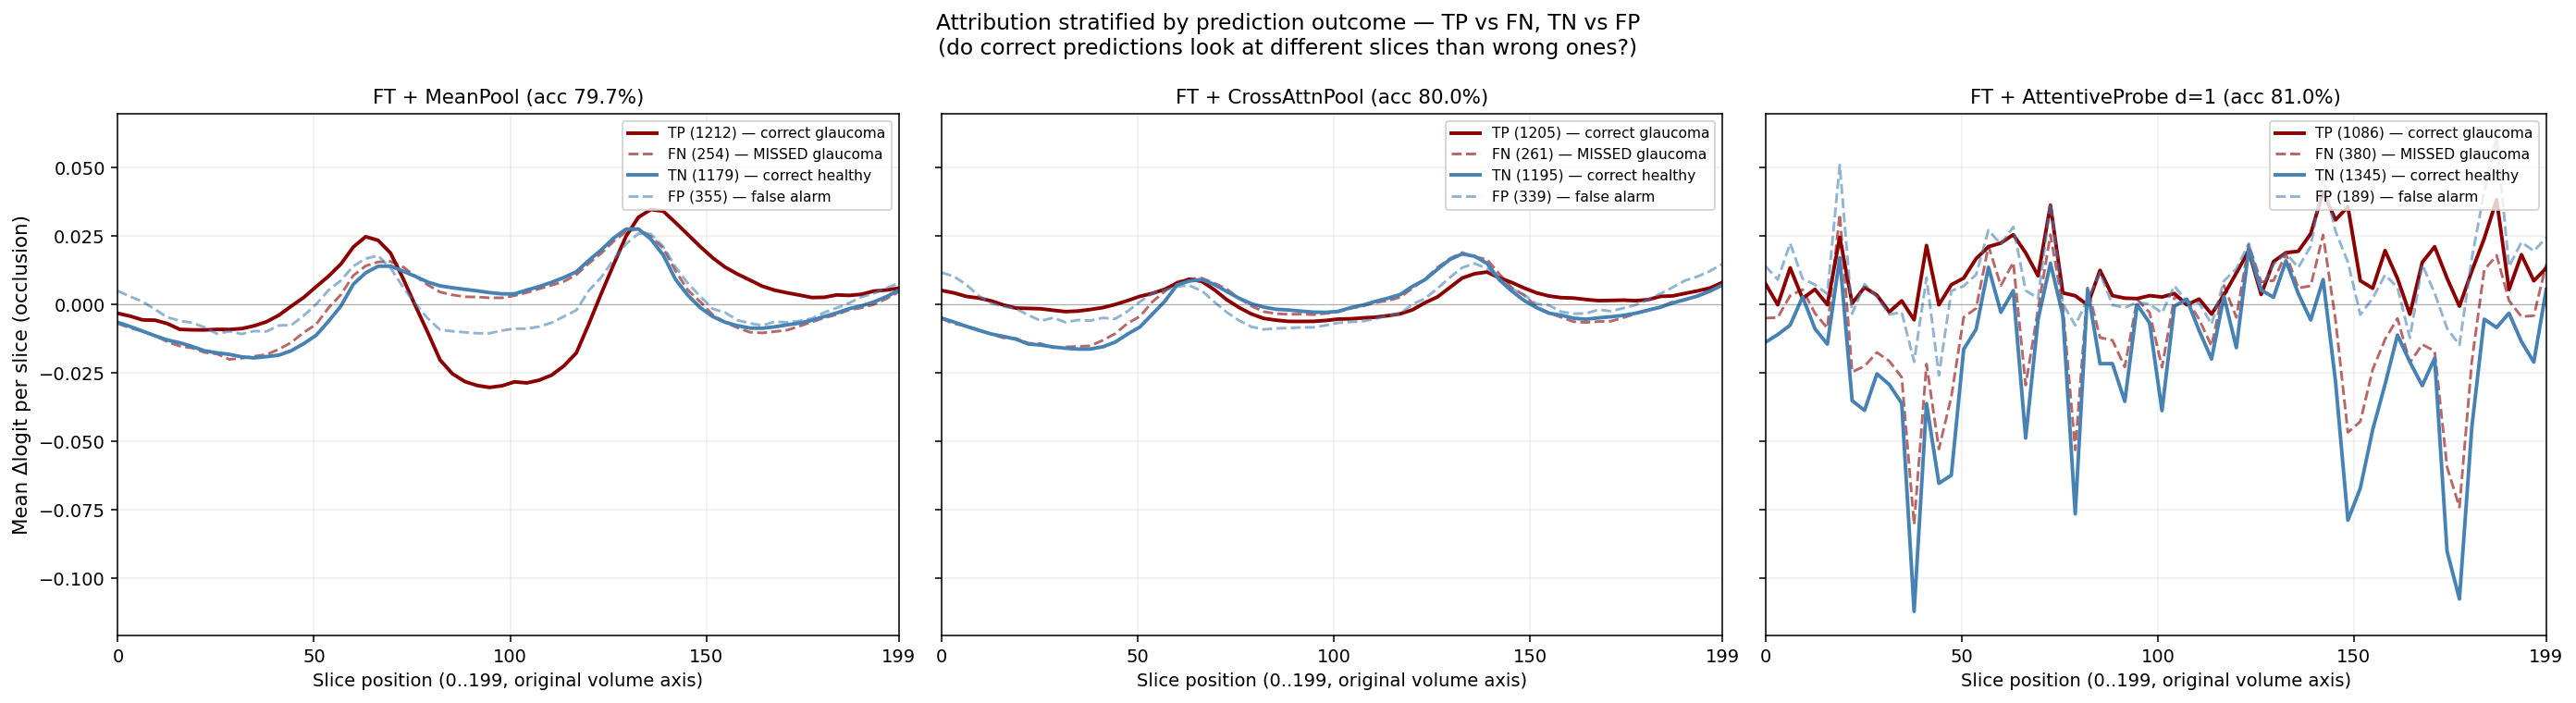
\includegraphics[width=0.92\linewidth]{interp_slice_contribution_by_outcome.png}
\caption{Attribution stratified by TP / FN / TN / FP. Errors reproduce the
correct pattern at lower amplitude rather than selecting different anatomy.}
\label{fig:interp-outcome}
\end{figure}

\begin{figure}[p]
\centering
\includegraphics[width=\linewidth,height=0.84\textheight,keepaspectratio]%
{interp_heatmap_grid.png}
\caption{Per-patch occlusion heat maps on individual B-scans, drawn on a shared
scale with the slice mean subtracted so that maps are comparable across volumes.
Attribution is broadly distributed
rather than concentrated in a few patches. Agreement is stronger at slice than
patch level.}
\label{fig:interp-heatmap}
\end{figure}

\paragraph{Diffuse attribution supports the main claim.} The classifier's
evidence is spread across the middle two-thirds
of the volume and across most patches within a slice
(Figure~\ref{fig:interp-heatmap}), rather than concentrated on
a compact anatomical target. A masking policy that sharpens targets onto a
precise anatomical boundary is therefore optimising for a spatial prior the
downstream task does not appear to need, which is consistent with
Section~\ref{sec:results-h3} finding no relationship between anatomical
specificity and downstream AUC. The OD/OS result is a methodological caution: a
figure that looks anatomically meaningful can be an artefact of data storage.

\section{Clinical operating points and calibration}
\label{app:operating}

AUC is threshold-free, but a screening tool is deployed at a threshold. The
threshold is selected on the \textsc{random} arm's \emph{validation} split at a
fixed target specificity and then applied unchanged to every arm on the test
split: one shared deployed threshold rather than a per-arm one, which simulates a
fielded screen and is conservative for the guided arms, since they are not
permitted to retune. The achieved test specificity shows whether the threshold
survives the shift. Cohort prevalence is $\Prevalence$.

\begin{table}[h]
\centering
\caption{Operating points at matched epoch 100. One threshold, chosen on the
\textsc{random} validation split to hit the target specificity, is applied
unchanged to all arms on test. ECE is a
15-bin expected calibration error.}
\label{tab:operating}
\small
\begin{tabular}{llcccccc}
\toprule
policy & target spec. & sens. & spec. (test) & PPV & NPV & Brier & ECE \\
\midrule
\textsc{random} & 0.85 & 0.7701 & 0.8259 & 0.8087 & 0.7899 & 0.1416 & 0.0355 \\
\textsc{random} & 0.90 & 0.7162 & 0.8794 & 0.8502 & 0.7643 & 0.1416 & 0.0355 \\
\textsc{envelope} & 0.85 & 0.7735 & 0.8351 & 0.8176 & 0.7942 & 0.1364 & 0.0361 \\
\textsc{envelope} & 0.90 & 0.7306 & 0.8807 & 0.8541 & 0.7738 & 0.1364 & 0.0361 \\
\ArmBest{} & 0.85 & 0.7851 & 0.8318 & 0.8169 & 0.8020 & 0.1341 & 0.0320 \\
\ArmBest{} & 0.90 & 0.7428 & 0.8696 & 0.8448 & 0.7797 & 0.1341 & 0.0320 \\
\bottomrule
\end{tabular}

\end{table}

Two observations (Table~\ref{tab:operating}). First, the threshold transfers
imperfectly: a validation target
of $0.90$ yields test specificity $\SpecAchIntensitySpecNinety$ to
$\SpecAchEnvelopeSpecNinety$ across the three arms, so the operating point moves
by roughly one point between arms and the comparison below is at a shared
threshold rather than at a shared false-positive rate.
Second, the AUC advantage survives as a usable sensitivity gain. At a target
specificity of $0.90$, \ArmBest{} detects $\SensIntensitySpecNinety$ of
cases against $\SensRandomSpecNinety$ for the unguided null, a paired difference
of $\DSensIntRandSpecNinety$ (CI $\DSensIntRandSpecNinetyCI$, excluding zero),
with the specificity caveat above. At
a target of $0.85$ the gain is $\DSensIntRandSpecEightyFive$
(CI $\DSensIntRandSpecEightyFiveCI$). \ArmBest{} is also the
best-calibrated arm (Brier $\BrierIntensity$ versus $\BrierRandom$; ECE
$\ECEIntensity$ versus $\ECERandom$), which matters because a screening score
that is used as a probability must be trustworthy as one.

A $+0.011$ AUC difference is hard to interpret clinically, and the ROC curves are
nearly superimposed (Figure~\ref{fig:roc}), whereas a change in cases detected at
a fixed threshold is not. We state that comparison carefully:
transferring one threshold moves achieved specificity from $\SpecAchRandomSpecNinety$
to $\SpecAchIntensitySpecNinety$, so the arms are \emph{not} compared at an
identical false-positive rate and the sensitivity change partly reflects that
shift. A deployment-grade comparison would select each arm's threshold on
validation to meet the same specificity, lock it, and evaluate on an untouched
cohort. One dataset, one split, one pretraining run per policy.

\paragraph{Who receives the benefit at the deployed threshold.} Subgroup AUC is
also threshold-free, so it cannot answer the question a deployment actually
raises: a screen ships \emph{one} threshold shared by everyone, and a model can
lift every subgroup's AUC while delivering the gain unevenly at that single
operating point. We therefore fix the threshold on validation at specificity
$\SOPSpecTarget$ ($\SOPThreshold$), transfer it unchanged, and measure the
change in sensitivity within each stratum
(Table~\ref{tab:subop}). Overall sensitivity rises from $\SOPSensRandom$ to
$\SOPSensOracle$.

The point estimates alone suggest the gain is concentrated in the largest group:
$\SOPDWhite$ for white patients against $\SOPDBlack$ for black patients, an
apparent ninefold difference. \textbf{The intervals do not support that reading.}
The black interval ($\SOPDBlackCI$) reaches almost exactly the white point
estimate, so the two are not separated; what distinguishes them is positive
count ($\SOPNWhitePos$ versus $\SOPNBlackPos$), not demonstrated benefit. Only
the white, female and male gains exclude zero, and those are the three largest
strata. This is a \emph{power} limitation of the cohort: the study cannot certify
that the smaller strata benefit, and equally cannot show they do not. Certifying
subgroup benefit at a deployed
threshold would need a cohort with more positives in the smaller strata.

\paragraph{The threshold itself does not transfer evenly across strata.} The
same table answers a question the sensitivity column does not. A threshold
selected on validation to achieve specificity $0.90$ does not achieve it
uniformly on test: under \textsc{random} it realises $0.895$ specificity in the
white stratum but $0.736$ in the black stratum, a shortfall of roughly sixteen
points, and under \ArmBest{} the same threshold realises $0.879$ and $0.761$.
The shortfall is therefore a property of transferring one threshold to a cohort
whose strata have different score distributions, and it is present under
\emph{both} arms; no masking policy here causes it and none of them repairs it.
For a screening context this is a larger effect than any AUC difference in this
paper.

\paragraph{The sensitivity gain is not a uniform trade.} Reporting sensitivity
alone would make the change from \textsc{random} to \ArmBest{} look like pure
benefit where it is in fact a trade. In the white stratum sensitivity rises by
$+0.034$ while specificity falls by $-0.016$; in the black stratum specificity
\emph{rises} by $+0.025$ and in the asian stratum by $+0.008$, alongside
sensitivity changes ($+0.004$ and $+0.008$) whose intervals contain zero. By
sex, both strata gain sensitivity ($+0.026$ female, $+0.027$ male) and lose
specificity ($-0.008$ and $-0.013$). Subgroup calibration moves the same way and
not entirely in our favour: expected calibration error improves overall
($\ECERandom$ to $\ECEIntensity$) and in the white ($0.0382$ to $0.0321$) and asian
($0.0832$ to $0.0729$) strata, but \emph{worsens} in the black stratum
($0.0525$ to $0.0569$). All values in these two paragraphs are measured at the
same shared threshold as Table~\ref{tab:subop}, and the comparison remains at a
shared threshold rather than at a shared realised false-positive rate.

\begin{table}[h]
\centering
\caption{Change in sensitivity from \textsc{random} to \ArmBest{} at one shared
deployed threshold (validation-selected, specificity $\SOPSpecTarget$), by
stratum. Paired bootstrap over positives within each stratum. Epoch 100.}
\label{tab:subop}
\small
\begin{tabular}{lcccc}
\toprule
stratum & positives & $\Delta$ sensitivity & 95\% CI & excludes 0 \\
\midrule
Asian & 118 & $+0.0085$ & $[-0.0339,\,+0.0508]$ & no \\
Black & 268 & $+0.0037$ & $[-0.0261,\,+0.0336]$ & no \\
White & 1080 & $+0.0343$ & $[+0.0194,\,+0.0491]$ & yes \\
Female & 811 & $+0.0259$ & $[+0.0074,\,+0.0444]$ & yes \\
Male & 655 & $+0.0275$ & $[+0.0092,\,+0.0458]$ & yes \\
\bottomrule
\end{tabular}

\end{table}

\begin{figure}[h]
\centering
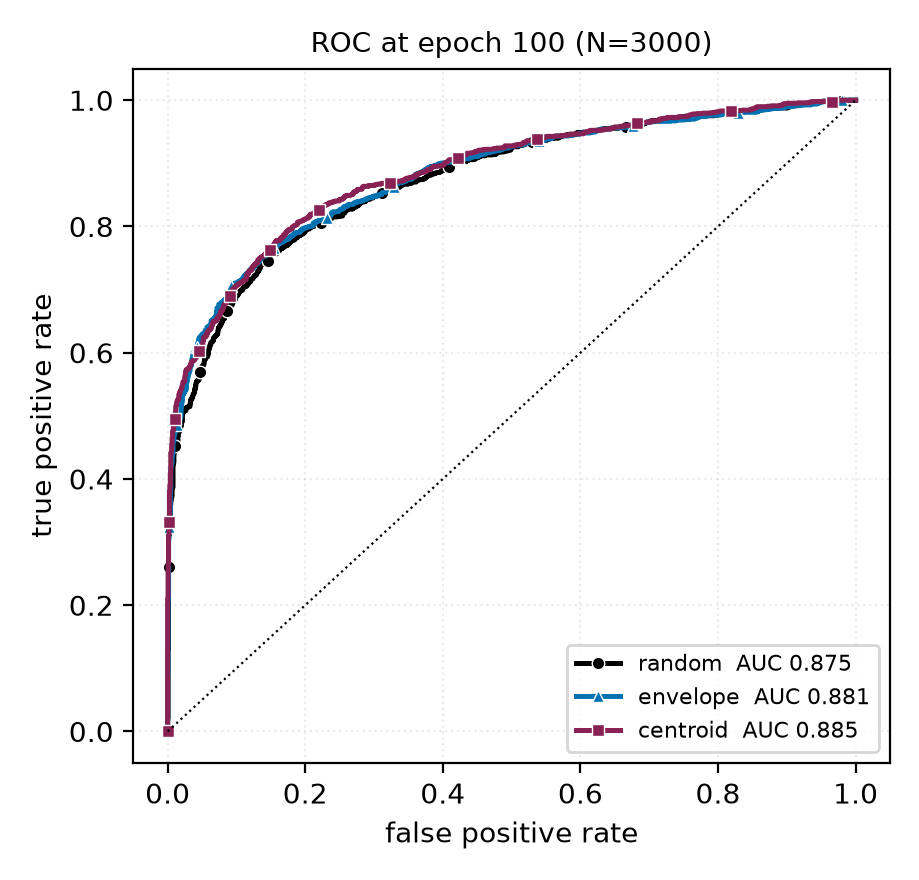
\includegraphics[width=0.62\linewidth]{fig_roc.png}
\caption{ROC curves at epoch 100 on the \Ntest{} test volumes. The three arms
plotted are nearly superimposed: the separation reported
throughout this paper is a small, consistent shift in the high-specificity
region rather than a difference visible in the curve as a whole. We include this
so the effect size is not overstated by tables alone.}
\label{fig:roc}
\end{figure}

\section{Broader impact and ethics}
\label{app:ethics}

This study uses a public, de-identified retinal dataset (FairVision) under its
release terms and involves no new data collection and no human subjects. No
model reported here is clinically validated or intended for deployment: the
frozen-probe AUCs are research measurements on one dataset and one task, and are
not evidence of clinical utility.

The subgroup analysis in Section~\ref{sec:subgroup} is a caution, not a
contribution. Every masking policy we tested leaves the same groups worst-served,
and the best-performing policy narrows none of them reliably, even though every subgroup point estimate rises at the matched
epoch. We would regard deployment
of any encoder reported here, without a dedicated and prospective fairness
evaluation on the target population, as inappropriate. We also stress that the
audit is incomplete: beyond AUC, the transferred-threshold sensitivity,
specificity and calibration of Appendix~\ref{app:operating}, and the race-by-sex
breakdown of Appendix~\ref{app:intersectional}, it contains no
predictive-value analysis and no subgroup calibration, and the intersectional
cells carry no paired per-cell intervals, so no per-cell change there is tested
against zero.

Releasing pretrained weights carries the usual dual-use consideration that they
may be applied to populations unlike the training cohort. We document the cohort
composition (Appendix~\ref{app:subgroup}) so that such a mismatch is detectable
by anyone reusing the weights. The demographic attributes are self-reported
categories inherited from the dataset's coding; they are used only for the
subgroup audit and are never model inputs.

\section{Published ablations on informed versus random masking}
\label{app:counter}

Our result should be read against the following published comparisons
(Table~\ref{tab:counter}), which we
collected while positioning this work. The pattern is that random masking is a
strong baseline and informed masking wins only under some objectives and
protocols; the deficit is largest under frozen evaluation.

\begin{table}[h]
\centering
\caption{Published ablations comparing a random or simple baseline against an
informed or structured masking scheme. Numbers are as reported by the cited
papers; metrics differ across rows and are not comparable between rows.}
\label{tab:counter}
\footnotesize
\setlength{\tabcolsep}{4pt}
\begin{tabular}{p{2.1cm}p{3.0cm}p{4.0cm}p{3.6cm}}
\toprule
study & baseline & informed variant & interpretation \\
\midrule
MAE~\citep{he2022mae} & random-75: 84.9 FT / 73.5 lin & block-75: 82.8 / 63.9; grid-75: 84.0 / 66.0 & random decisively better \\
SimMIM~\citep{xie2022simmim} & 83.0 top-1 & best block 82.7; square 82.6 & random modestly better \\
SemMAE~\citep{li2022semmae} & random 66.8 lin & within-part 66.5; whole-part 52.9; adaptive 68.7 & naive semantics hurt; scheduled semantics help \\
SemMAE part quality~\citep{li2022semmae} & no parts 63.7 & raw parts 63.6; refined 65.0 & an imperfect semantic model adds nothing \\
AutoMAE~\citep{chen2023automae} & MAE 83.26 FT & AutoMAE 83.32 & effectively tied \\
HPM~\citep{wang2023hpm} & random 82.49 & moderate 82.95; hardest-only 81.40 & benefit only with retained randomness \\
AttMask~\citep{kakogeorgiou2022attmask} & random 43.4 $k$-NN & high 43.5; hint 43.6 & nearly indistinguishable \\
AttG-MAE~\citep{sick2025attg} & MAE 78.5 @10\% labels & guided 78.1 & guidance loses in this protocol \\
SSiT~\citep{huang2024ssit} & no saliency 79.48 $\kappa$ & 25\% mask 77.53; 50\% 79.97 & dataset-dependent, non-monotonic \\
\bottomrule
\end{tabular}
\end{table}

Read together, these say that the \emph{direction} of our finding is not new.
What we add is the controlled measurement, not the sign of the result.

\section{Full paired-contrast table}
\label{app:contrasts}

\begin{table}[t]
\centering
\caption{Primary contrasts: matched epoch \emph{and} matched precision. $\Delta$
is a paired difference on identical test cases; the interval is a
\Nboot-resample paired bootstrap and $p$ is a DeLong test for correlated ROC
curves. $q$ is Benjamini--Hochberg over these nine contrasts. All $p$ and $q$
values here are descriptive (Section~\ref{sec:limits}).
Every comparison against the null excludes zero.}
\label{tab:contrasts}
\small
\begin{tabular}{llcccc}
\toprule
contrast & epoch & $\Delta$ AUC & 95\% CI & $p$ & $q$ \\
\midrule
\textsc{envelope} $-$ \textsc{random} & 50  & \DEnvelopeRandomEpFifty  & \DEnvelopeRandomEpFiftyCI  & \DEnvelopeRandomEpFiftyP  & \DEnvelopeRandomEpFiftyQ \\
\textsc{envelope} $-$ \textsc{random} & 75  & \DEnvelopeRandomEpSeventyFive  & \DEnvelopeRandomEpSeventyFiveCI  & \DEnvelopeRandomEpSeventyFiveP  & \DEnvelopeRandomEpSeventyFiveQ \\
\textsc{envelope} $-$ \textsc{random} & 100 & \DEnvelopeRandomEpHundred & \DEnvelopeRandomEpHundredCI & \DEnvelopeRandomEpHundredP & \DEnvelopeRandomEpHundredQ \\
\addlinespace
\ArmBest{} $-$ \textsc{random}   & 50  & \DOracleRandomEpFifty    & \DOracleRandomEpFiftyCI    & \DOracleRandomEpFiftyP    & \DOracleRandomEpFiftyQ \\
\ArmBest{} $-$ \textsc{random}   & 75  & \DOracleRandomEpSeventyFive    & \DOracleRandomEpSeventyFiveCI    & \DOracleRandomEpSeventyFiveP    & \DOracleRandomEpSeventyFiveQ \\
\ArmBest{} $-$ \textsc{random}   & 100 & \DOracleRandomEpHundred   & \DOracleRandomEpHundredCI   & \DOracleRandomEpHundredP   & \DOracleRandomEpHundredQ \\
\addlinespace
\ArmBest{} $-$ \textsc{envelope} & 50  & \DOracleEnvelopeEpFifty  & \DOracleEnvelopeEpFiftyCI  & \DOracleEnvelopeEpFiftyP  & \DOracleEnvelopeEpFiftyQ \\
\ArmBest{} $-$ \textsc{envelope} & 75  & \DOracleEnvelopeEpSeventyFive  & \DOracleEnvelopeEpSeventyFiveCI  & \DOracleEnvelopeEpSeventyFiveP  & \DOracleEnvelopeEpSeventyFiveQ \\
\ArmBest{} $-$ \textsc{envelope} & 100 & \DOracleEnvelopeEpHundred & \DOracleEnvelopeEpHundredCI & \DOracleEnvelopeEpHundredP & \DOracleEnvelopeEpHundredQ \\
\bottomrule
\end{tabular}
\end{table}

Benjamini--Hochberg is applied within a declared confirmatory family consisting
of exactly these nine contrasts --- the fp16 comparisons among \textsc{random},
\ArmBest{} and \textsc{envelope} at epochs 50, 75 and 100 --- and the remaining
25 exploratory contrasts in the stored statistics are corrected as a separate
family. The two families are never pooled, and the $q$ values printed above are
those of the nine-contrast family only.

\section{Full fp32 re-probe}
\label{app:fp32}

\begin{figure}[h]
\centering
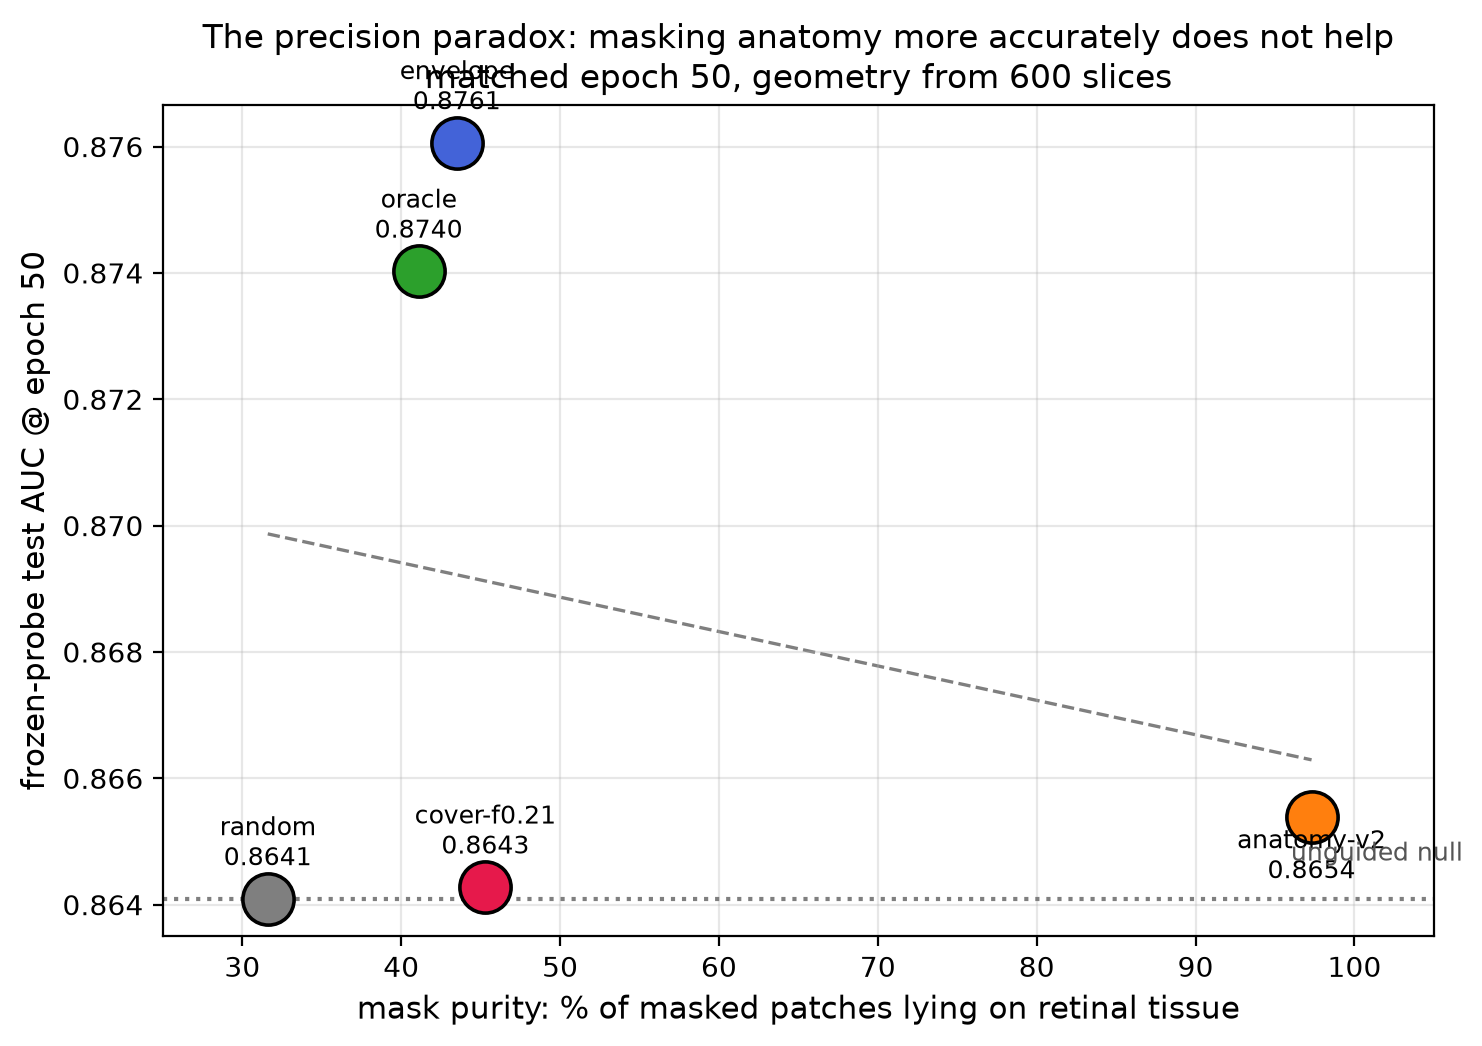
\includegraphics[width=0.46\linewidth]{fig_precision_paradox.png}
\caption{Downstream AUC at matched epoch 50 against mask purity, the fraction of
masked patches lying on retinal tissue. The policy whose masks are $97\%$
on-tissue does not separate from the null, while policies at $40$--$43\%$ purity
gain the most. The ordering does not support the intuition that more accurate
anatomical masking yields better representations. With four to five arms this is
descriptive, not inferential.}
\label{fig:paradox}
\end{figure}

\begin{figure}[h]
\centering
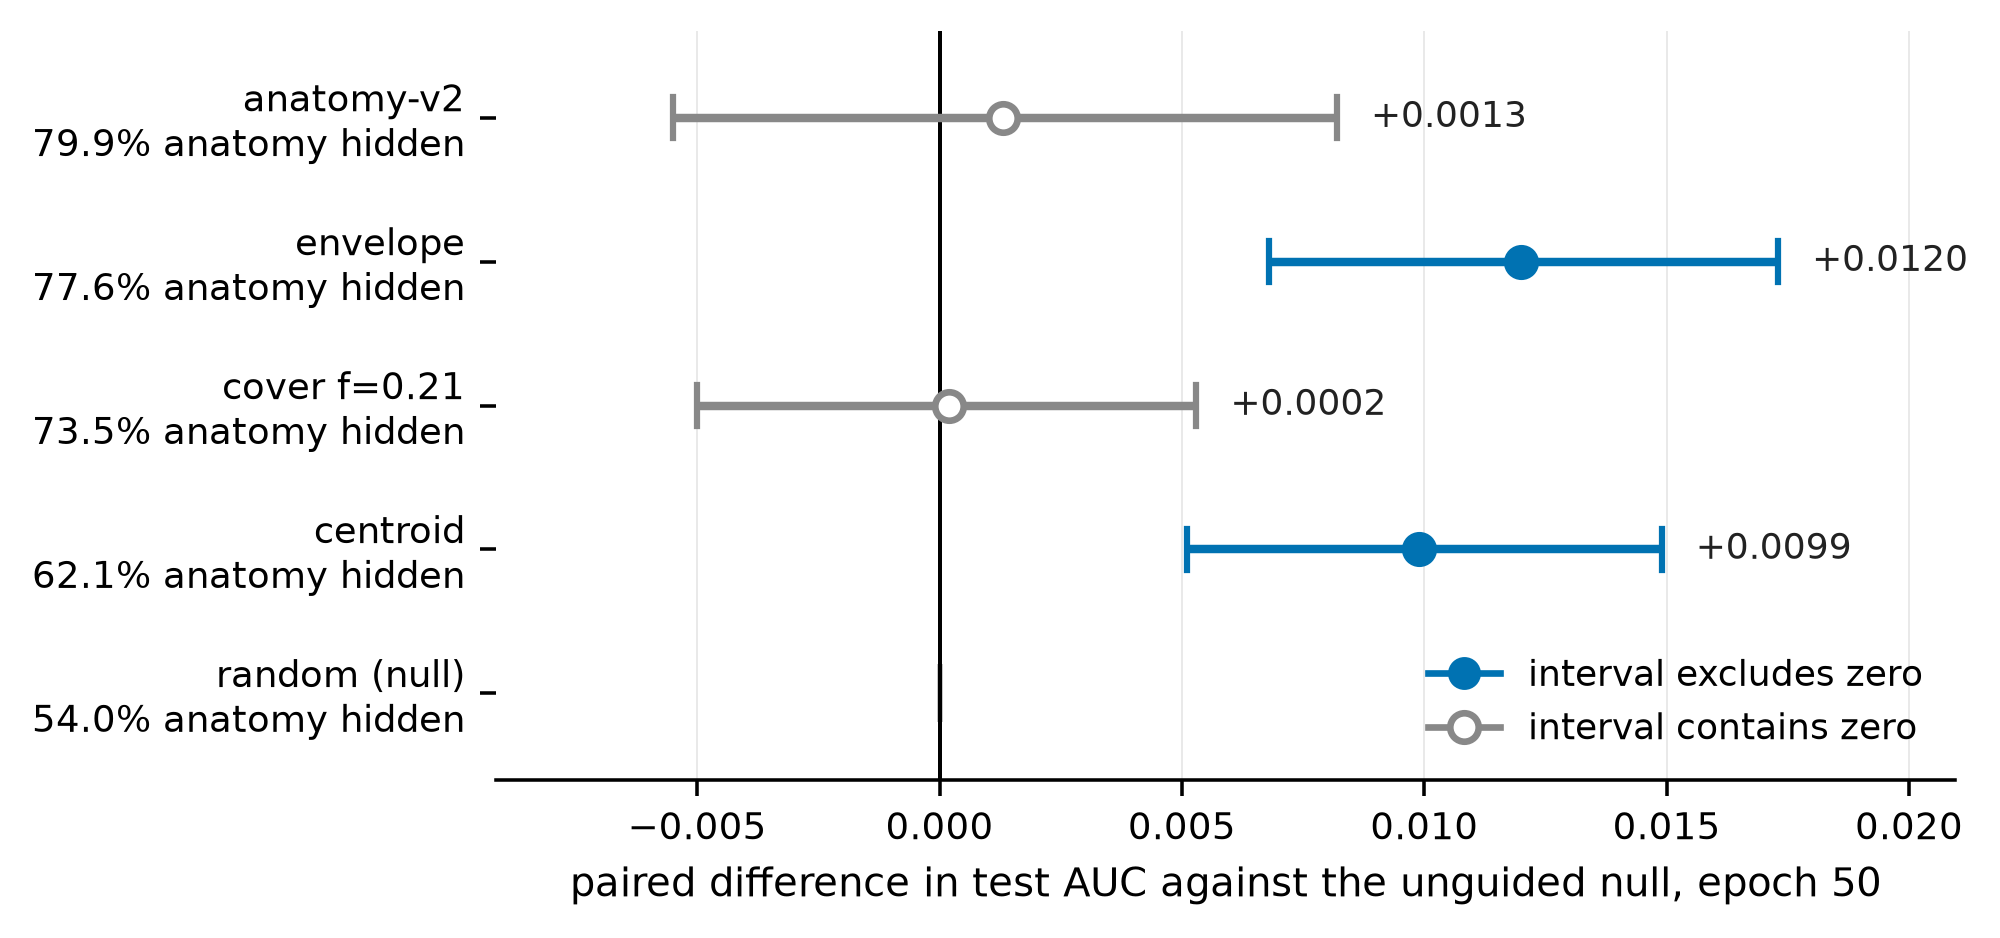
\includegraphics[width=0.6\linewidth]{fig_specificity_ladder.png}
\caption{The matched-epoch-50 result arranged as a ladder of increasing
anatomical specificity. Companion to Figure~\ref{fig:paradox}.}
\label{fig:ladder}
\end{figure}

\begin{figure}[h]
\centering
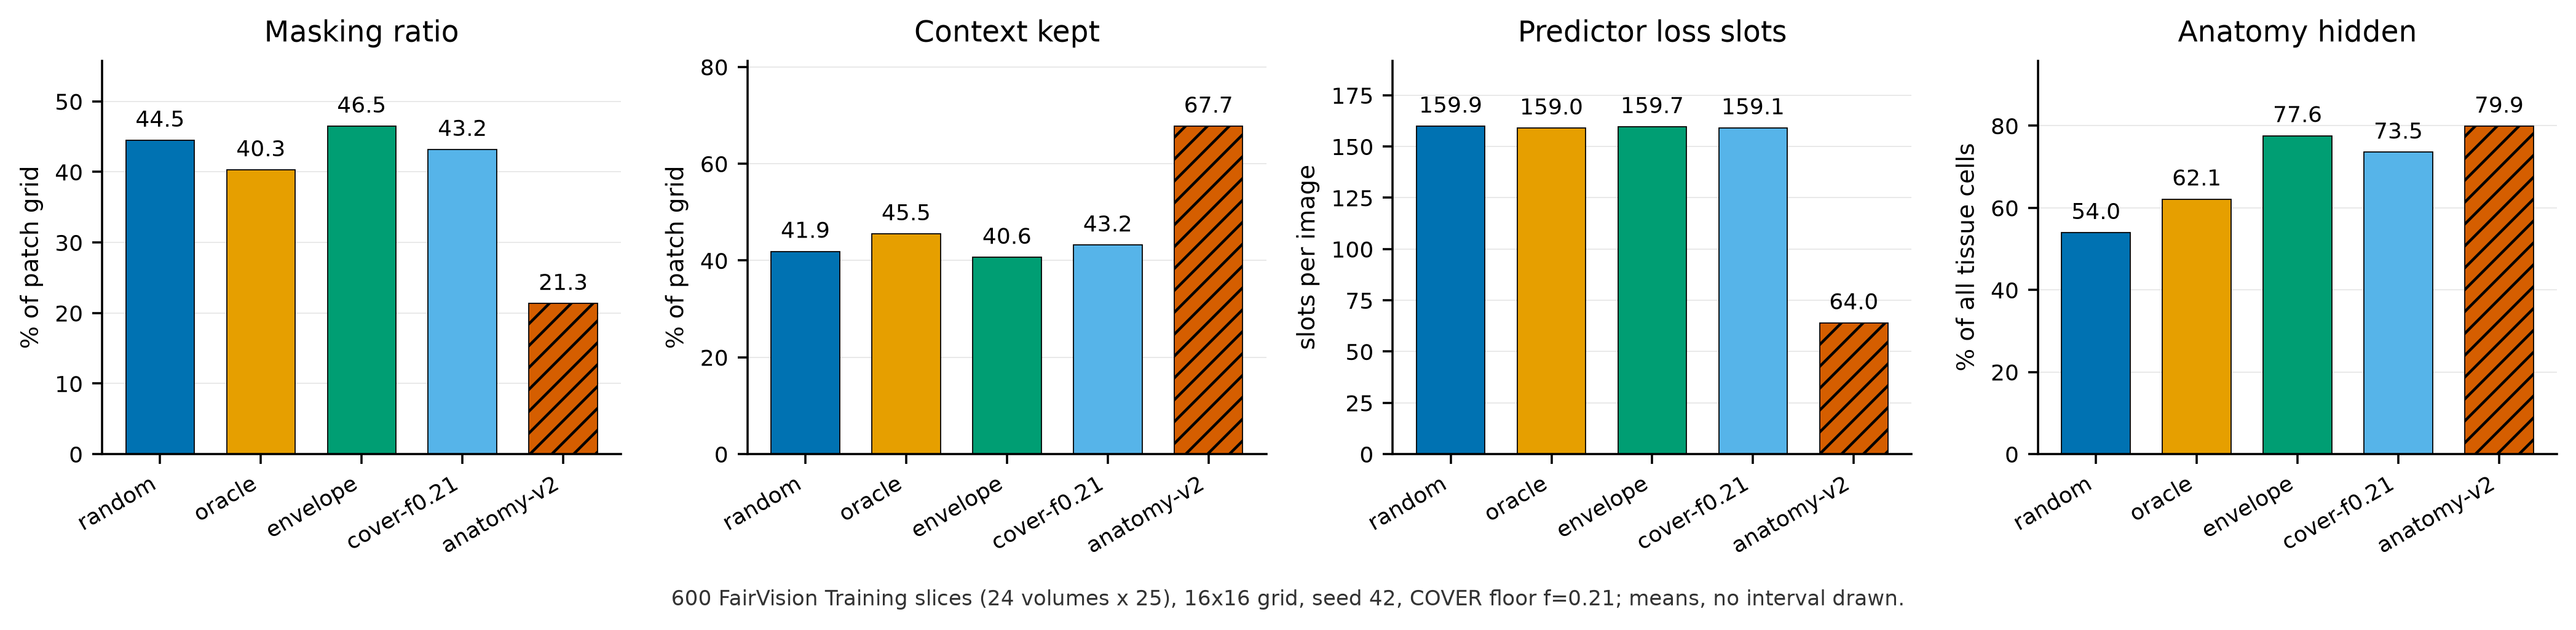
\includegraphics[width=\linewidth]{fig_geometry_panel.png}
\caption{Measured mask geometry per policy, 600 training slices. The four
rectangle policies are closely matched on every axis, so their comparison is
near single-variable. The anatomy policy diverges on all four simultaneously ---
half the masking ratio, $1.6\times$ the context, $0.4\times$ the predictor loss
slots --- so its deficit cannot be attributed to target shape.}
\label{fig:geom}
\end{figure}

The \textsc{random}, \ArmBest{} and \textsc{envelope} long-horizon probes
were originally fitted under the harness default, which enables autocast. To
remove any doubt that the headline effect is a precision artifact, we re-ran the
complete probe pipeline for those arms with autocast disabled, so that feature
extraction, head optimisation and test evaluation are all fp32, under the exact
protocol already used by the \textsc{anatomy} and \textsc{cover} arms
(Table~\ref{tab:fp32}). The
encoder checkpoint is SHA-256 hashed before and after each run and verified
unchanged, so no result here can be contaminated by an accidental encoder
update.

\begin{table}[h]
\centering
\caption{Full fp32 re-probe against the original fp16 result, same frozen
encoder in each row. The largest difference is $2\times10^{-4}$, two to three
orders of magnitude below the effects reported in Table~\ref{tab:main}.}
\label{tab:fp32}
\small
\begin{tabular}{lccccc}
\toprule
policy & epoch & fp16 AUC & fp32 AUC & $\Delta$ & $p$ \\
\midrule
\textsc{envelope} & 50 & 0.876064 & 0.876063 & -0.000001 & 0.964 \\
\textsc{envelope} & 100 & 0.880743 & 0.880761 & +0.000018 & 0.167 \\
\textsc{oracle} & 100 & 0.885485 & 0.885293 & -0.000192 & 0.767 \\
\textsc{random} & 100 & 0.874581 & 0.874485 & -0.000096 & 0.000 \\
\bottomrule
\end{tabular}

\end{table}

\section{Reproducibility and numeric provenance}
\label{app:repro}

\paragraph{Guide provenance differs across the segmenter arms.} The three
segmenter-driven policies do not all read the same anatomy guide.
\textsc{envelope} samples the unmodified MIRAGE occupancy map.
\textsc{anatomy-v1} and \textsc{cover} instead read pre-computed \emph{soft}
guides produced by a MIRAGE whose segmentation path carries a frozen residual
adapter, trained label-free to align MIRAGE's patch-similarity structure with the
pretraining teacher's. That adapter was an abandoned line of work --- it reduced
its own training objective but never improved segmentation, and the experiment
that would have settled its downstream effect was not run --- so we make no claim
about it here. We record it because it is a further axis on which the anatomy
arms and \textsc{cover} differ from \textsc{envelope}, beyond the geometric axes
in Section~\ref{sec:results-h3}, and because the guide directory names embed the
adapter configuration and would otherwise be unexplained to anyone reproducing
this work. \ArmBest{} and \textsc{random} consult no guide of either kind.

\paragraph{What is checked mechanically.} Every quantity in this paper resolves
through a generated macro file produced by one script from stored per-case
predictions, so prose, tables and figures cannot disagree. Three further gates
run on every build: a consistency check that fails on an undefined or duplicated
macro, a dangling reference or citation, or a banned overclaiming phrase; a
provenance check that resolves each AUC macro's arm and epoch from its own name
and fails if the value does not match that arm's stored probe, which makes
reporting one arm's number under another arm's name a build error; and an
archive check that compiles the submission from a clean extraction and enforces
the page limit and anonymity.

\paragraph{Checkpoint identity.} The shared epoch-25 ancestor is identified by
SHA-256
(\texttt{e5ad5b0c2aadfa15449409786afbfa39d8b5405b699be8f02f2e540195e97e7b}),
which three independent copies reproduce, and the replication chain of
Appendix~\ref{app:replication} re-hashes it before each leg. Every frozen probe
hashes its encoder before and after fitting and invalidates the run if the hash
moves, so no reported probe can have been contaminated by an accidental encoder
update. The six replication configurations are generated by a script that
asserts they differ only in the seed and logging fields.

\paragraph{An audit of hand-typed numbers, and what it found.} Generated macros
are verified by the gates above; numbers typed directly into the manuscript
source are not, and that gap is where our errors have been. We therefore audited
every numeric quantity typed into the source: 310 occurrences, of which 234 were
confirmed against a stored artifact, 75 had no producing artifact that we could
locate, and one was wrong --- a probe parameter count quoted for the wrong probe
configuration, since corrected. Two unbacked quantities carried interpretive
weight: a per-cell concentration statistic used to argue that the best arm was
the most spatially consistent, and a probe-seed noise bound. Both have been
removed from this version rather than restated, and the mechanism claim that
rested on the first has been withdrawn with it (Sections~\ref{sec:results-h3}
and~\ref{sec:limits}). The rule we adopted, and recommend, is that a numeric
claim which is not machine-generated is treated as unverified until it is
recomputed.

\section{Fine-tuning narrows but does not erase the gap}

Under full fine-tuning rather than a frozen probe, \ArmBest{} reaches
$\FTOracleMeanpool$ (mean-pool head) against \textsc{random}'s
$\FTRandomMeanpool$, a gap of $\FTDelta$ compared with $\DOracleRandomEpHundred$
frozen. Taking each arm's best head instead, the gap is $\FTDeltaBest$. The
pretraining difference is partially, but not entirely, absorbed by supervised
adaptation --- consistent with the masking policy shaping the representation
rather than merely the optimisation start point. These runs used a different
head and schedule from the frozen probes and are never pooled with them.


\section{Fine-tuned results}

\begin{table}[h]
\centering
\caption{Full fine-tuning, same test split. Reported separately from frozen
probes and never pooled with them.}
\small
\begin{tabular}{llc}
\toprule
policy & head & test AUC \\
\midrule
\ArmBest{} & mean-pool & 0.894668 \\
\ArmBest{} & cross-attention & 0.893717 \\
\ArmBest{} & attentive & 0.890100 \\
\textsc{random} & attentive & 0.887763 \\
\textsc{random} & cross-attention & 0.887178 \\
\textsc{random} & mean-pool & 0.886756 \\
\bottomrule
\end{tabular}
\end{table}

\end{document}
